\documentclass[a4paper,12pt, openright, oneside]{book}
%\usepackage{setspace}
%\singlespacing
%\onehalfspacing
\usepackage[T1]{fontenc}
\usepackage[utf8]{inputenc}
\usepackage{setspace}
\usepackage{geometry}
\usepackage{subcaption}
\usepackage{amsmath}

\DeclareMathOperator*{\argmax}{argmax} 
\DeclareMathOperator*{\argmin}{argmin} 


\usepackage{wrapfig}

\usepackage{natbib}
\bibliographystyle{acl_bib_style}

\usepackage[most]{tcolorbox}
\usepackage{subfig} %For subcaptions

\newcommand{\mysubfig}[3][width=\linewidth]{%
    \tcbitem\subfloat[#2]{\includegraphics[#1]{#3}}}

\usepackage[english]{babel}
%\usepackage{enumitem}
\usepackage[final]{pdfpages}
\usepackage[colorlinks=true,allcolors=blue]{hyperref}%
\usepackage{caption}
\usepackage{graphicx}
\usepackage{amsmath,amsfonts,amssymb}
\usepackage{tabularx, tabulary, array}
\usepackage{algorithm,algpseudocode}
\usepackage{multirow}
\usepackage{booktabs}

\usepackage{todonotes}

% \usepackage{lineno}
% \linenumbers

\usepackage[inline, shortlabels]{enumitem}
\setlist{itemjoin ={,\enspace},itemjoin* = { and\enspace}}


\newcolumntype{C}{>{\centering\arraybackslash}X}

\graphicspath{{images/}}

\pagestyle{plain} 

\begin{document}

\begin{titlepage}
    \newgeometry{margin=1in}    
    \noindent
    \begin{minipage}[t]{0.19\textwidth}
        \vspace{-4mm}{
\includegraphics[scale=1.15]{images/logo_unimib.pdf}}
    \end{minipage}
    \begin{minipage}[t]{0.81\textwidth}
    {
            \setstretch{1.42}
            {\textsc{Università degli Studi di Milano - Bicocca}} \\
            \textbf{Scuola di Scienze} \\
            \textbf{Dipartimento di Informatica, Sistemistica e Comunicazione} \\
            \textbf{Corso di laurea in Informatica} \\
            \par
    }
    \end{minipage}
    
\vspace{40mm}
    
\begin{center}
        {\LARGE{
                \setstretch{1.2}
                \textbf{Zero-Shot Cross-Language Relation Extraction as Multilingual Machine Comprehension}
                \par
        }}
    \end{center}
    
    \vspace{40mm}

    \noindent
    {\large \textbf{Relatore:} Dott. Elisabetta Fersini} \\

    \noindent
    {\large \textbf{Correlatore:} Prof. Anders S{\o}gaard}
        
    \vspace{15mm}

    \begin{flushright}
        {\large \textbf{Relazione della prova finale di:}} \\
        \large{Cezar Angelo Sas} \\
        \large{Matricola 781563} 
    \end{flushright}
        
    \vspace{40mm}
    \begin{center}
        {\large{\bf Anno Accademico 2018-2019}}
    \end{center}

    \restoregeometry
        
\end{titlepage}

\restoregeometry


\pagenumbering{roman}

{\hypersetup{linkcolor=black}
\tableofcontents
}




\clearpage
\pagenumbering{arabic}

\chapter{Introduction}
\paragraph{}

With the advent of the internet, a large amount of digital text is produced each day as news articles, research publications, blogs, and social media. It is essential to advance techniques for automatically extracting information from these documents, as much valuable knowledge is hidden within them. This extracted information can be used to enhance access and management of knowledge hidden in large text corpora. The computer science field that concerns the processing of natural language is called Natural Language Processing (NLP). 

However, most of this information is produced only in English; indeed, it is a widely lamented fact that linguistic and encyclopedic resources are heavily biased towards English. Even multilingual knowledge bases (KBs) such as Wikidata \citep{vwikidata} are predominantly English-based \citep{Kaffee:Simperl:18}. This suggests that coverage is higher for English and that facts of interest to English-speaking communities are more likely included in a KB.

This also means that current natural language processing research and development has mainly focused on English. Recognizing this, the community has in recent years put emphasis on multilingual and cross-lingual resources and methods which allow for the joint exploitation of resources between languages and for the transfer of models from well-resourced languages to lower-resourced ones.

In this work, we discuss such problems in the context of Relation Extraction (RE), which is an Information Extraction (IE) subtask. IE is a field that concerns NLP, computational linguistic, and data mining. The goal of IE is to extract structured information from a collection of unstructured documents, this is achieved via different subtask like named entity recognition, coreference resolution, and relation extraction. Relation extraction consists of identifying mentions of the relations of interest in each sentence of the given documents, the extracted relation are then used to populate knowledge bases. Traditional relation extraction system are required to only extract seen relations, which make easier to train these models as the data required can be obtained via crowd sourcing~\citep{liu-etal-2016-effective} or distant supervision~\citep{hoffmann-etal-2011-knowledge}. These models are meant to generalize to new entities, but {\em not} new {\em relations}. In this work, we consider the  case in which models are trained on a subset of pre-specified relations and applied to both seen and unseen entities, and unseen relations. The latter scenario is known as {\em zero-shot} RE \citep{rocktaschel2015injecting}.

As a possible solution to this problem,~\cite{levy2017zero} propose an alternative approach to the relation extraction task. By reframing the problem as question answering, they can use reading comprehension techniques that allow zero-shot relation extraction. 

Our interest in multilingual relation extraction concerns three different questions: \begin{enumerate}[a) , font=\bfseries, noitemsep]
    \item how well relation extraction models can be transferred across different languages?
    \item can the variance in the number of relations examples between languages help  build more robust relation extraction models?
    \item can a jointly trained model that performs RE on multiple languages perform equally or better than the monolingual trained version?
\end{enumerate}

Unfortunately, as aforementioned, there is a lack of multilingual resources, and this is also true for  relation extraction. For the best of our knowledge, there is no large corpora for multilingual relation extraction available. The only resource contains around 90K examples and it is available only in three languages. To solve this and answer our questions, based on~\citep{levy2017zero, hewlett2016wikireading} we propose \textbf{X-WikiRE}, a new multilingual resource for relation extraction as question answering and using state-of-the-art models we investigate how such resource can be used in different transfer learning scenarios. By performing various experiments we show how our multilingual resource helps both in case of low resource languages by performing sequential transfer learning, and also that \textbf{X-WikiRE} improves the performances on single languages when jointly training a single model on multiple languages.



% This work explores techniques for automatically filling such language gaps by learning to add facts in other languages, and more generally shows that multilingual sharing is beneficial for knowledge base completion. 


\paragraph{}
This work is organized through the following chapters: in Chapter~\ref{chpt:2} we present some natural language processing and machine learning concepts and methodologies background. In Chapter~\ref{chpt:3} we present the state of the art in relation extraction and machine comprehension. Next, Chapter~\ref{chpt:4} presents \textbf{X-WikiRE}, our new multilingual relation extraction dataset; while in Chapter~\ref{chpt:5} we describe the used machine comprehension model and our experimental setup. Finally, in Chapter~\ref{chpt:6} we present the results obtained using our dataset. To conclude, Chapter~\ref{chpt:7} contains some final thoughts and future developments.
\chapter{Background}
\label{chpt:2}
\paragraph{}
This chapter provides an overview of the different task and concepts needed to perform relation extraction in a multilingual setup. Some concepts, like Word Representation~(Section \ref{sec:word_embedding}) are at the core of NLP, while others are more general machine learning techniques (Section~\ref{sec:nn},~\ref{sec:transfer_learning} and \ref{sec:zero_learning}), some others instead are both general and have a very high usage in NLP due to their nature (Section \ref{sec:sequence_modeling}). After a brief description of each of these concepts, we will focus on their application in NLP in particular for relation extraction. In the next Chapter we will describe more the task of relation extraction, and present how Natural Language Understanding, a sub-field of NLP that deals with machine reading comprehension, can be used for relation extraction.

% \section{Introduction}
% Natural Language Processing solutions span form rule based systems~\citep{brill-1992-simple, nebhi2013rulere}, to statistical approaches~\citep{skounakis2003hierarchical}, and also to neural networks~\citep{pawar-etal-2017-end}.

\section{Neural Networks}
\label{sec:nn}

\paragraph{}
A Neural Network (NN) is a computational model inspired by networks of biological neurons, wherein the neurons compute output values from inputs. The simplest form of neural network is the feed forward neural network, in which the information flows only in one direction, and there is no recurrent connection between the nodes. Neural networks try to approximate some function $f^{*}$ by defining a mapping $y = f(x; W)$ for an input $x$ and learning the value of the parameters $W$ that yield the best function approximation. A neural network is called network because they contain multiple layers of artificial neurons. The artificial neuron is the building block of neural networks.

A neuron is defined by an input $x$, a set of weights $W$, a bias $b$, and an activation function $g$. The activation function should be differentiable, since to actually learn, we need to compute derivatives. With $x, W \in \mathbb{R}^{n\times1}$, $b \in \mathbb{R}$. The output $y$ is defined as: 

\begin{equation}
    y = g(W^{\intercal} x + b)
\end{equation}


Feed forward neural networks are composed by various layers, each layer contains some neurons. The formal definition is very similar to the one of the neuron. We will include the bias term in the weights matrix, and have an extra element $x_0 = 1$ in the input $x$. Given a feed forward neural network with $L$ layers, the forward propagation is: 

\begin{equation}
\begin{split}
    %y = f^{k}(W_{k}^{\intercal} * \dots f^{2}(W_{2}^{\intercal} * f^{1}(W_{1}^{\intercal} * x)) \dots)
    z & = W^{i-1}a^{i-1} \\
    a^{i} & = g(z^i) \\
    y & = a^L g(z^L) \\
\end{split}
\end{equation}

Where $g$ is an activation function, $a^i$ is the activation of layer $i$, and $a^0 = x$. The weight matrix $W_i$ controls the mapping from layer $i$ to layer $i+1$. Given a network with $s_i$ units in layer $i$, and $s_{i+1}$ in layer $i+1$ the weight matrix $W_i \in\mathbb{R}^{(s_{i+1})\times (s_i + 1)} $. And the final prediction is $y = a^{L}$. 

As in other machine learning algorithms, we have to learn the parameters of our neural network. We have a cost function, or objective function, $J(\theta)$ that we try to minimize. Given a neural network $h_\theta$, we compute our cost function as a sum of the error function  $\mathcal{L}$ for all the examples. The error function computes the difference between the predicted value $\hat{y} = h_{\theta}(x)$ and the actual value $y$. We also have a regularizer term $\Omega$ that is weighted by the hyperparameter $\lambda$:

\begin{equation}
    \min_{\theta} J(\theta) = - \frac{1}{N} \sum_{1}^{N} \mathcal{L}(y_i, \hat{y_i}) + \lambda \Omega_\theta
\end{equation}

Now that we have defined what is the goal of our neural network, we can start performing the training. %The learning algorithm for neural network is called backpropagation, from backward propagation of errors. 
The weights $\theta$ in the network are the only parameters that can be modified to make the cost function $J$ as low as possible; thus we can minimize $J$ by using an iterative process of gradient descent, for which we need to calculate the gradient for the cost function with respect to the network parameters.  As each network consists of various layers, computing the gradient of the loss function w.r.t the parameters $\frac{\partial J}{\partial \theta}$ is non-trivial. To estimate the gradient, we use a an algorithm called backpropagation~\citep{rumelhart1988learning}, from backward propagation of errors. As the name implies, backpropagation starts computing the gradients from the output of the networks and moves backward to the input through all layers. First, we need to compute the derivative of $J(\theta)$ w.r.t the output, this will be our $\partial^{L}$, then go backward:



%Equation~\ref{eq:backpropagation}. 

\begin{equation}
\begin{split}
    \partial^{L} & = \frac{\partial}{\partial y} \mathcal{L}(y, \hat{y}) \\
    \partial^i &= {\theta^{i}}^\intercal \partial^{i+1} \odot \left(\frac{\partial}{\partial z^{i}} g(z^i)\right)
\end{split}
\label{eq:backpropagation}    
\end{equation}

For each layer, the computed gradients are then used to update the corresponding parameters using gradient descent.

\section{Sequence Modeling}
\label{sec:sequence_modeling}


\paragraph{}
Due to the inherent nature of natural language almost all NLP tasks deal with sequences. For example, in speech recognition, we have the input audio which is a sequence of phonemes that will be recognised and used to produce a transcript. Likewise, in machine translation where we have as input a sequence of words in a source language and the machine has to generate a sequence of words with the same meaning of the one in input but in a target language.


Traditional neural networks are not designed to deal with the temporal information of sequences in an efficient way. A way to handle this problem is to introduce the notion of a dynamical system. In the dynamical system, there is a state which carries information about past inputs. Typically, we make what is called a Markov assumption; that means that all the information regarding the past and current inputs required to estimate a future state is succinctly contained in the current state. A Recurrent Neural Network is a particular type of dynamical system.

\subsection{Recurrent Neural Network}
\paragraph{}
The most elementary neural network for sequential input is the recurrent neural network~\citep{elman1990finding}. Elman proposes a recurrent network based on the idea introduced by~\citet{jordan1986} which proposes a network with recurrent connections from the output to the input; these are one-to-one connections that are used to associate a static pattern with a serially ordered output pattern. Elman modifies the network by moving the recurrent connection. Instead of having the output connected with the input, Elman adds additional units at the input level, these units are called ``\textit{context units}'' are connected to the hidden layer. Context units are also “hidden” in the sense that they interact exclusively with other nodes internal to the network, and not the outside world. 

In Figure~\ref{fig:rnn} we can have a look at how a RNN works. The network $A$ takes in input $x_t$ and produces an output $h_t$, a loop enables the information to flow from the previous step to the current, allowing the prediction to be affected by the last state of the network. A more effective way to think about RNNs is by unrolling them (right side of Figure~\ref{fig:rnn}). We can formally define $A$ as:

\begin{figure}[t]
        \centering
        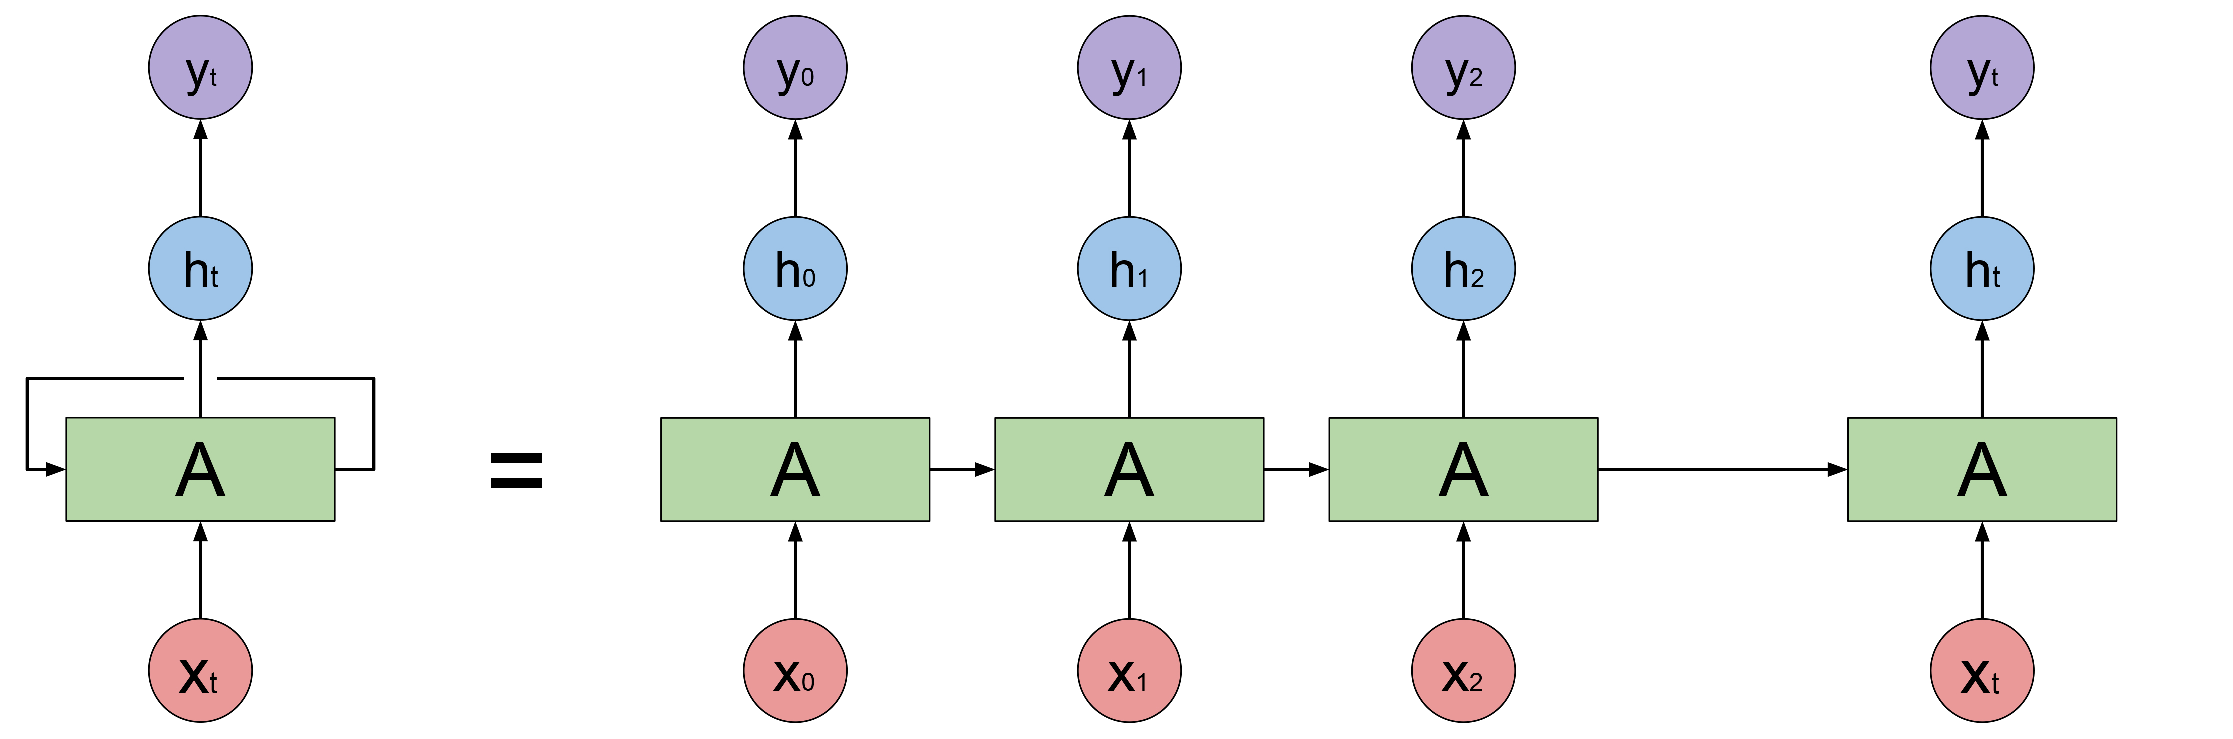
\includegraphics[width=0.9\textwidth]{images/RNN_with_prediction.pdf}
        \caption{RNN unrolling. On the left a compact representation of RNNs, on the right the same RNN can be unrolled}
        \label{fig:rnn}
\end{figure}%

\begin{equation}
\begin{split}
    h_t & = f_W(h_{t-1}, x_t) \\
    y_t & = g_{\theta}(h_t)
\end{split}
\label{eq:generic_rnn}
\end{equation}

Where, $h_t$ is the new state, $f_W$ and $g_\theta$ are functions with parameters $W$ and $\theta$ respectively, $h_{t-1}$ is the previous state, $x_t$ is the current input, and $y_t$ is the output at the \textit{t-th} step.
The vanilla RNN is defined using a neural network with $\tanh$ as activation function, so we will have:

\begin{equation}
\begin{split}
    h_t & = \tanh\left(W_h \cdot h_{t-1} + W_x \cdot x_t\right)\\
        & = \tanh\left([W_h, W_x] \cdot \begin{bmatrix}
           h_{t-1} \\
           x_t
         \end{bmatrix}\right)\\
         & = \tanh\left(W \cdot \begin{bmatrix}
           h_{t-1} \\
           x_t
         \end{bmatrix}\right)
\end{split}
\end{equation}

Where $W_h$, $W_x$ are weights for the hidden and input respectively. 

\paragraph{}
RNN are able to manage variable length of input and output sequences, we can have different types of RNN according to these sizes. Given a sequence $x$ of length $l_x$, and a desired output sequence $y$ with length $l_y$, we can define the following types (visually represented in Figure~\ref{fig:rnn_types}):

\begin{enumerate}[a), noitemsep]
    \item One-to-One: $l_x = l_y = 1$, this is a traditional neural network;
    \item One-to-Many: $l_x = 1, l_y > 1$, this is the case for sequence generation;
    \item Many-to-One: $l_x > 1, l_y = 1$, for sequence classification;
    \item Many-to-Many: $l_x = l_y > 1$, for sequence labeling;
    \item Many-to-Many: $l_x \neq l_y, l_x > 1, l_y > 1$, also referred to as sequence to sequence~\citep{sutskever2014sequence}, or encoder-decoder~\citep{cho-etal-2014-learning}. Given an input sequence, the encoder process it and generates a dense representation, usually the last hidden state, that is used to initialize the decoder that will produce the output sequence.
\end{enumerate}

\begin{figure}
\begin{tcbitemize}[
    raster columns=3,
    raster halign=center,
    raster every box/.style={blankest}
    ]
\mysubfig{One-to-One}{images/one_to_one.pdf}
\mysubfig{One-to-Many}{images/one_to_many.pdf}
\mysubfig{Many-to-One}{images/many_to_one.pdf}
\mysubfig{Many-to-Many}{images/many_to_many.pdf}
\mysubfig{Many-to-Many}{images/many_to_many_s2s.pdf}
\end{tcbitemize}

\caption{Different types of RNN}
\label{fig:rnn_types}
\end{figure}

% \begin{figure} [H]
% \centering
% \begin{tabular}{cccc}
% 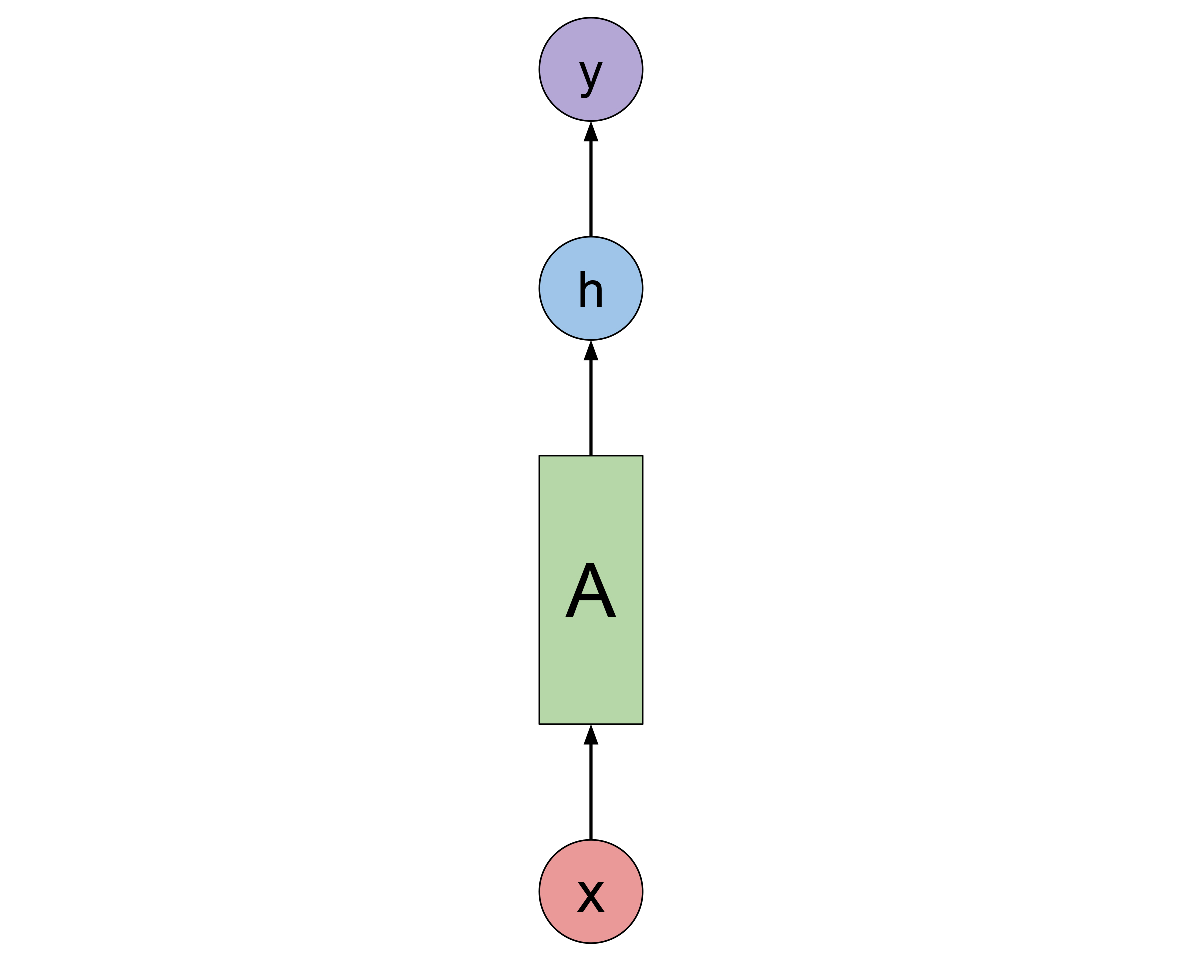
\includegraphics[width=0.3\textwidth]{images/one_to_one.pdf} &
% 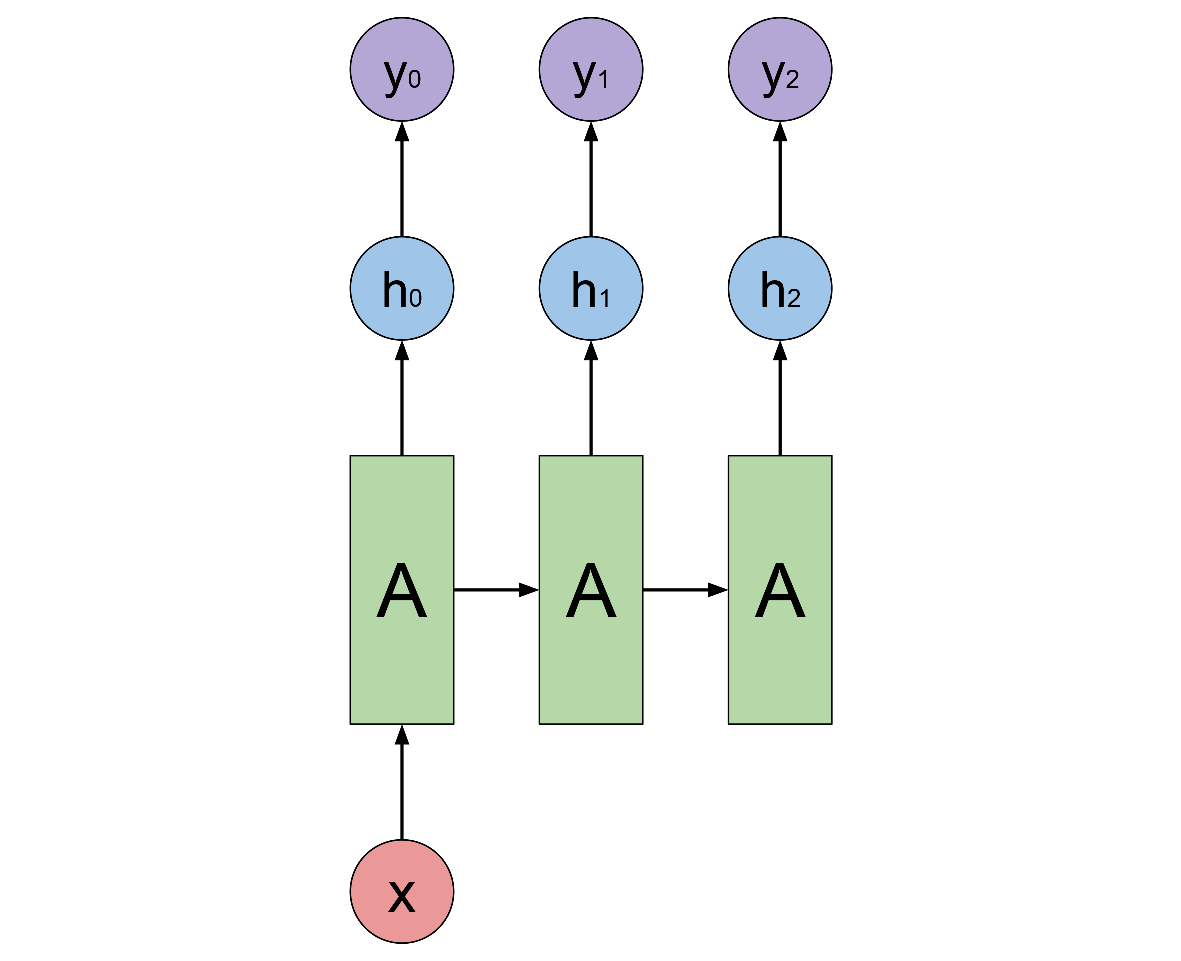
\includegraphics[width=0.3\textwidth]{images/one_to_many.pdf} &
% 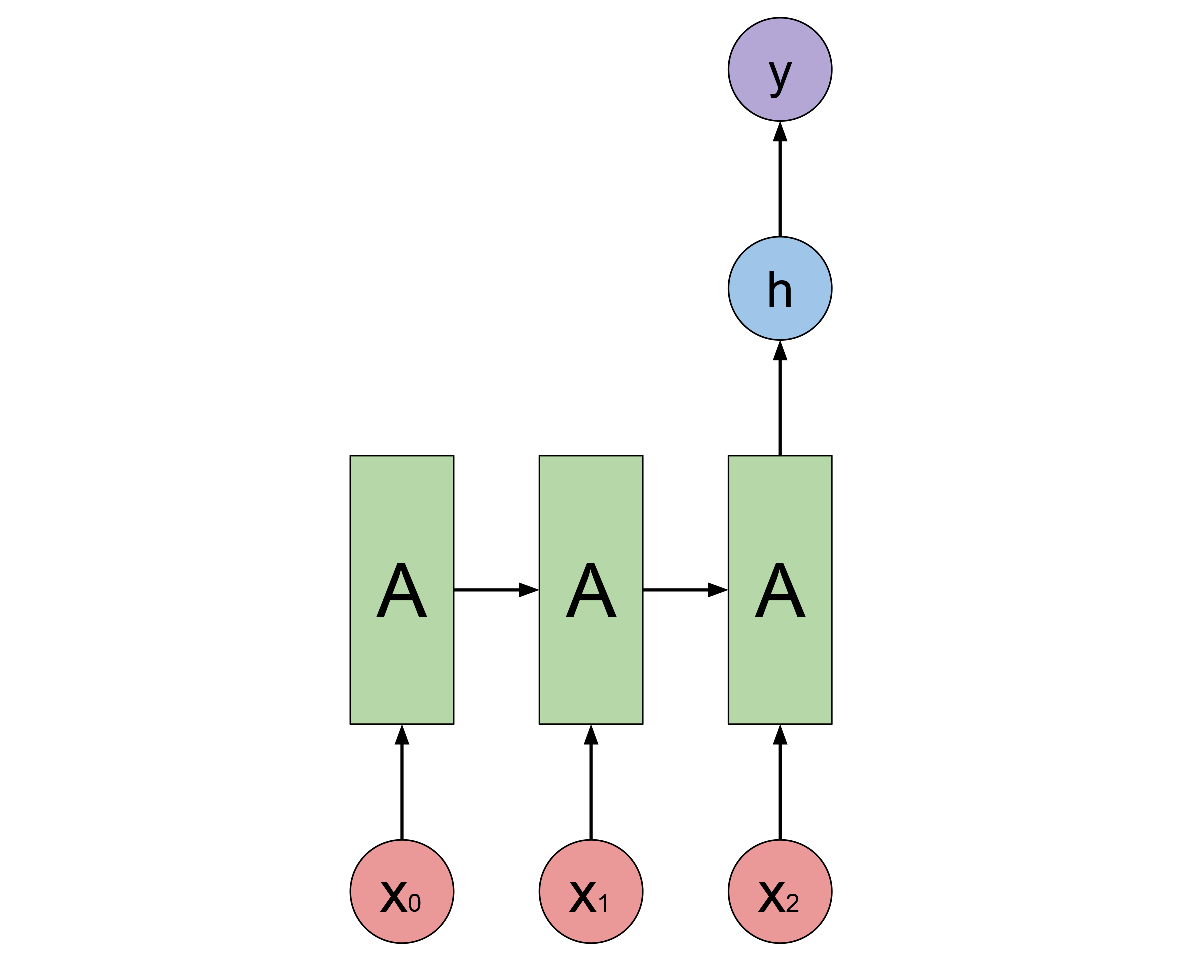
\includegraphics[width=0.3\textwidth]{images/many_to_one.pdf} \\
% \textbf{(a)}  & \textbf{(b)} & \textbf{(c)}  \\[6pt]
% \end{tabular}
% \begin{tabular}{cccc}
% \includegraphics[width=0.3\textwidth]{example-image-a} &
% \includegraphics[width=0.3\textwidth]{example-image-b} \\
% \textbf{(d)}  & \textbf{(e)}  \\[6pt]
% \end{tabular}
% \caption{ \textbf{(a)} Some text
% \textbf{(b)} Some text
% \textbf{(c)} Some text
% \textbf{(a)} Some text
% \textbf{(b)} Some text}
% \label{fig:peroxide}
% \end{figure}

% \begin{table}[ht]
% \caption{A table arranging  images}
% \centering
% \begin{tabular}{*{4}{|m{0.24\textwidth}}|}
% \hline
% 1 & 2 & 3 & 4  \\
% \hline
%  \begin{center}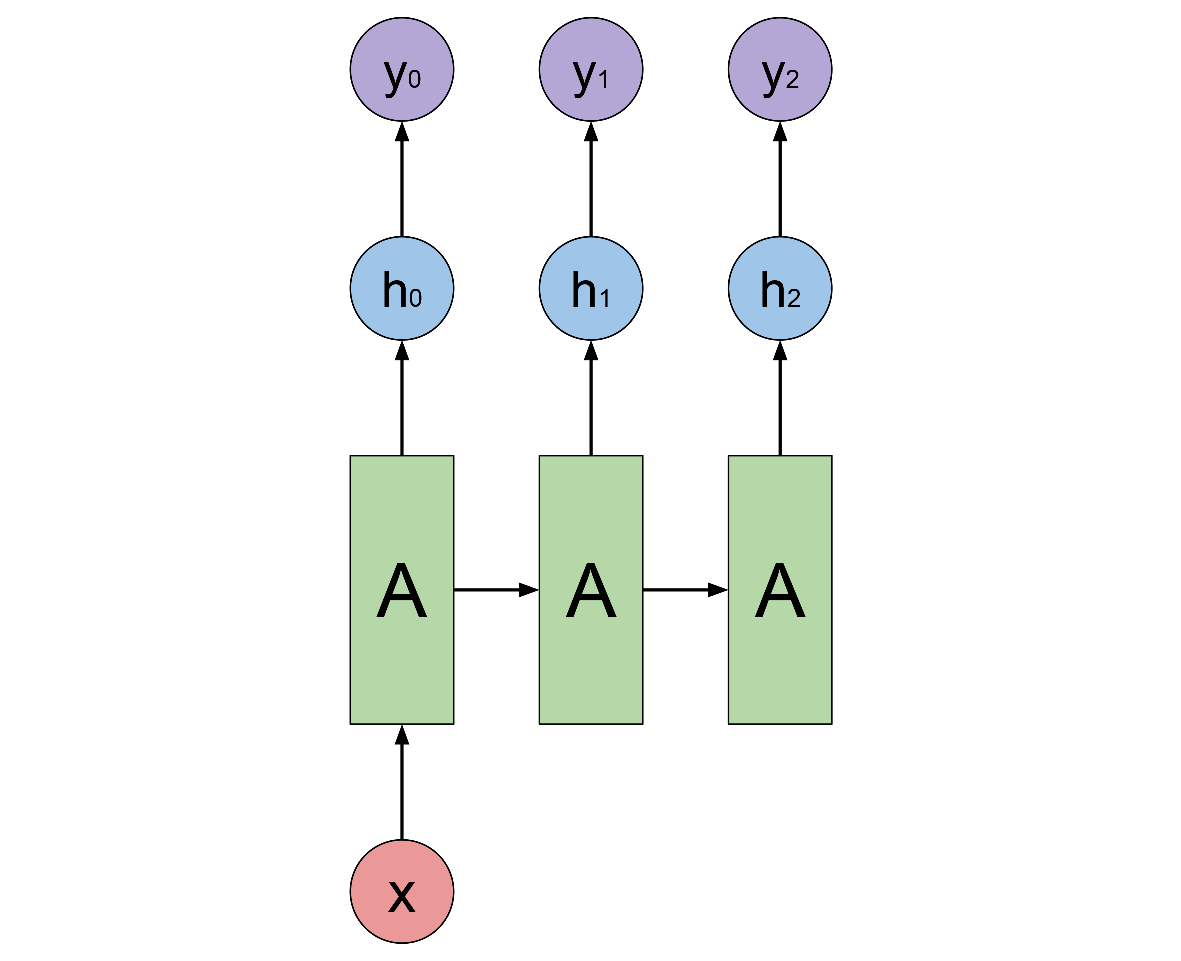
\includegraphics[height=0.1\textwidth]{images/one_to_many.pdf} \end{center} &
% \begin{center}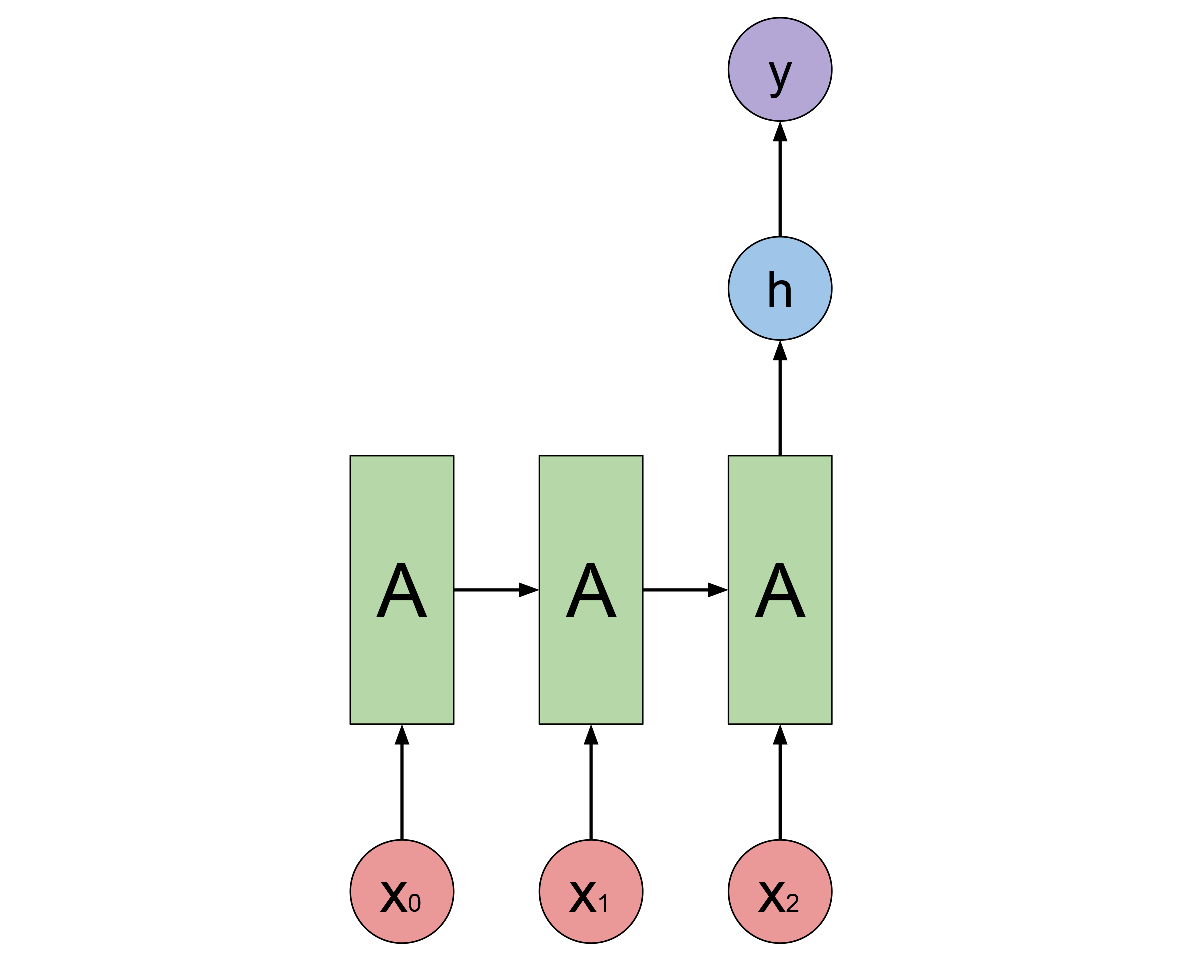
\includegraphics[height=0.1\textwidth]{images/many_to_one.pdf} \end{center} &
% \begin{center}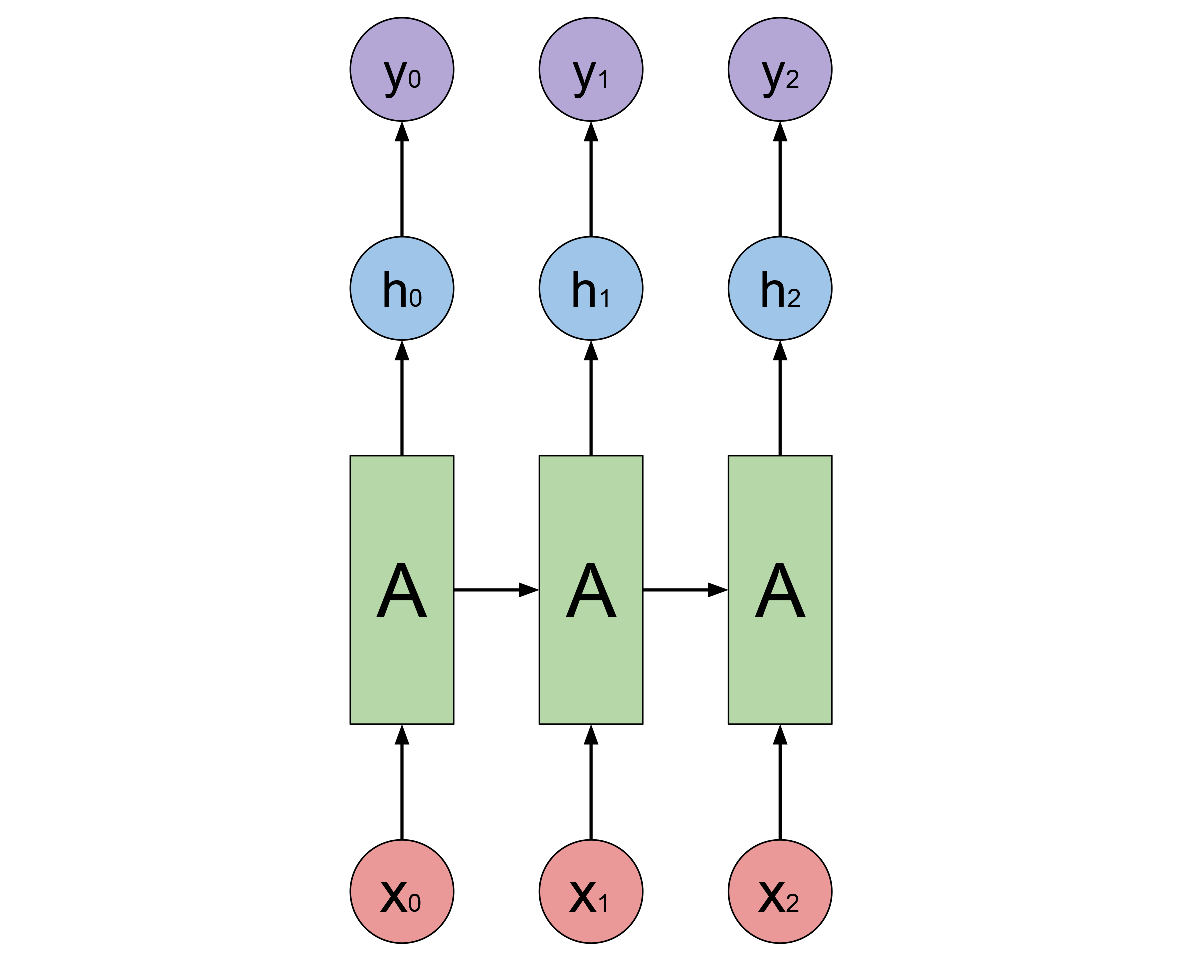
\includegraphics[height=0.1\textwidth]{images/many_to_many.pdf} \end{center} & \begin{center}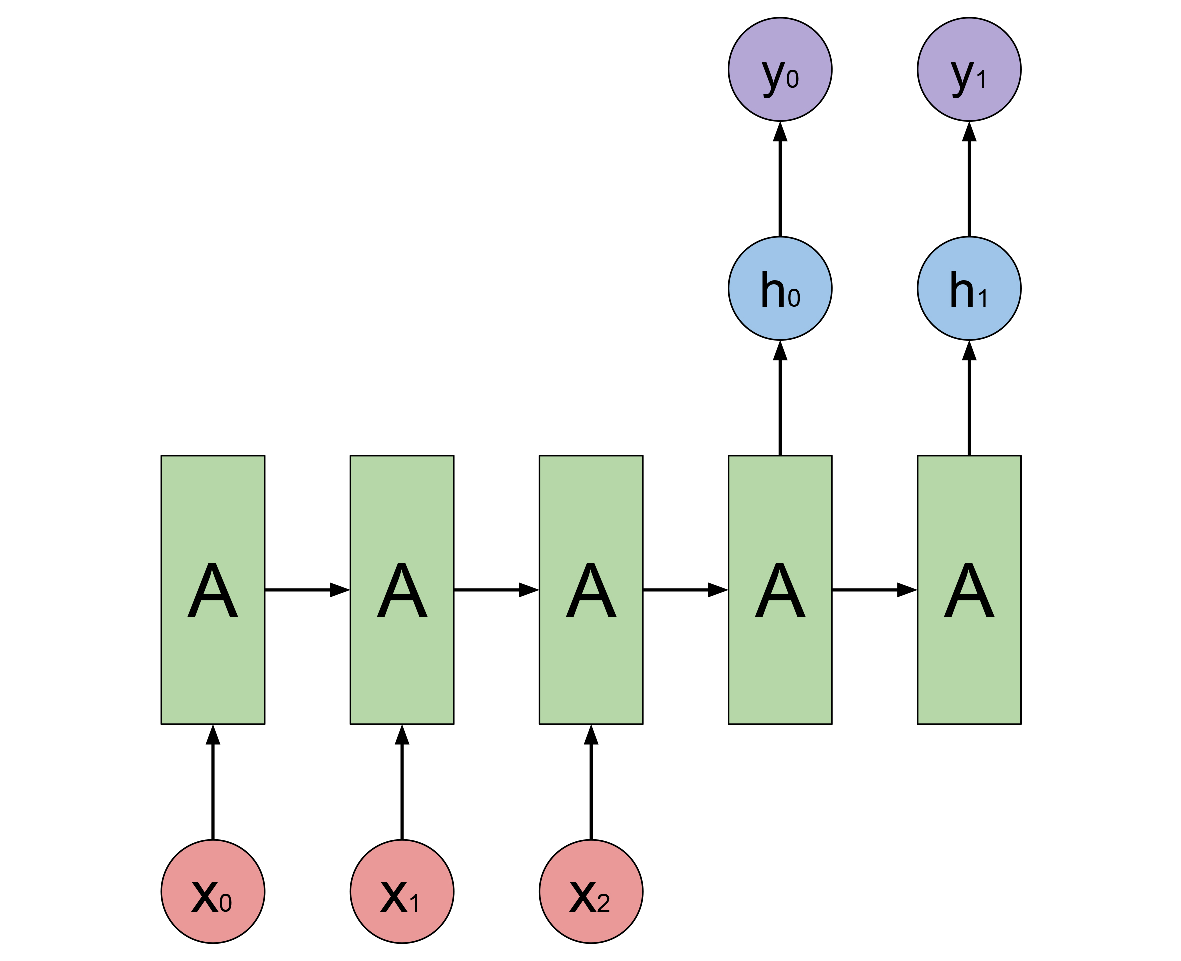
\includegraphics[height=0.1\textwidth]{images/many_to_many_s2s.pdf} \end{center} \\
% \hline
% \end{tabular}
% \label{tab:gt}
% \end{table}

% \begin{table}[ht]
% \caption{A table arranging  images}
% \centering
% \begin{tabular}{*{4}{|m{0.24\textwidth}}|}
% \hline
% This is some text & \begin{center}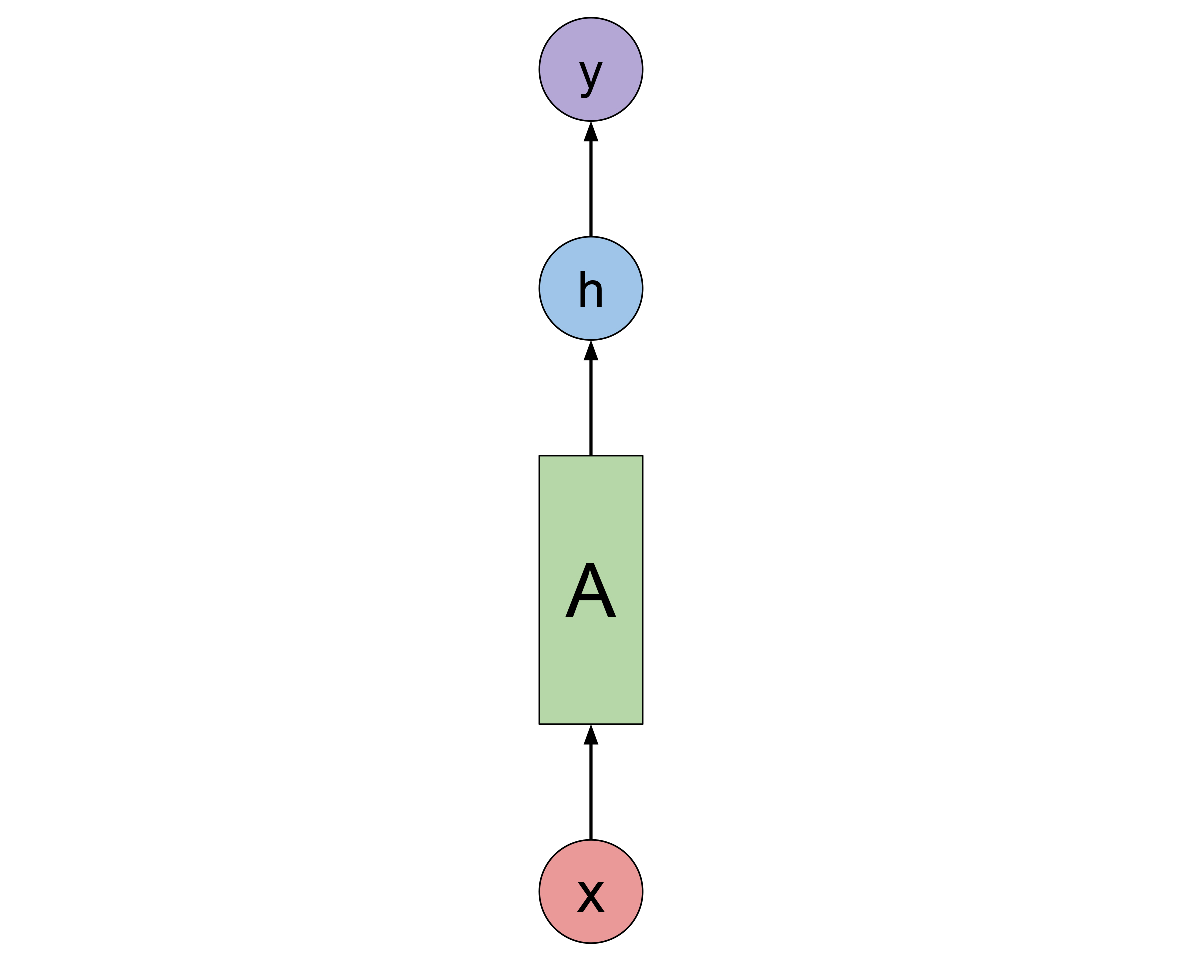
\includegraphics[height=0.2\textwidth]{images/one_to_one.pdf}\end{center} & This is some text & \begin{center}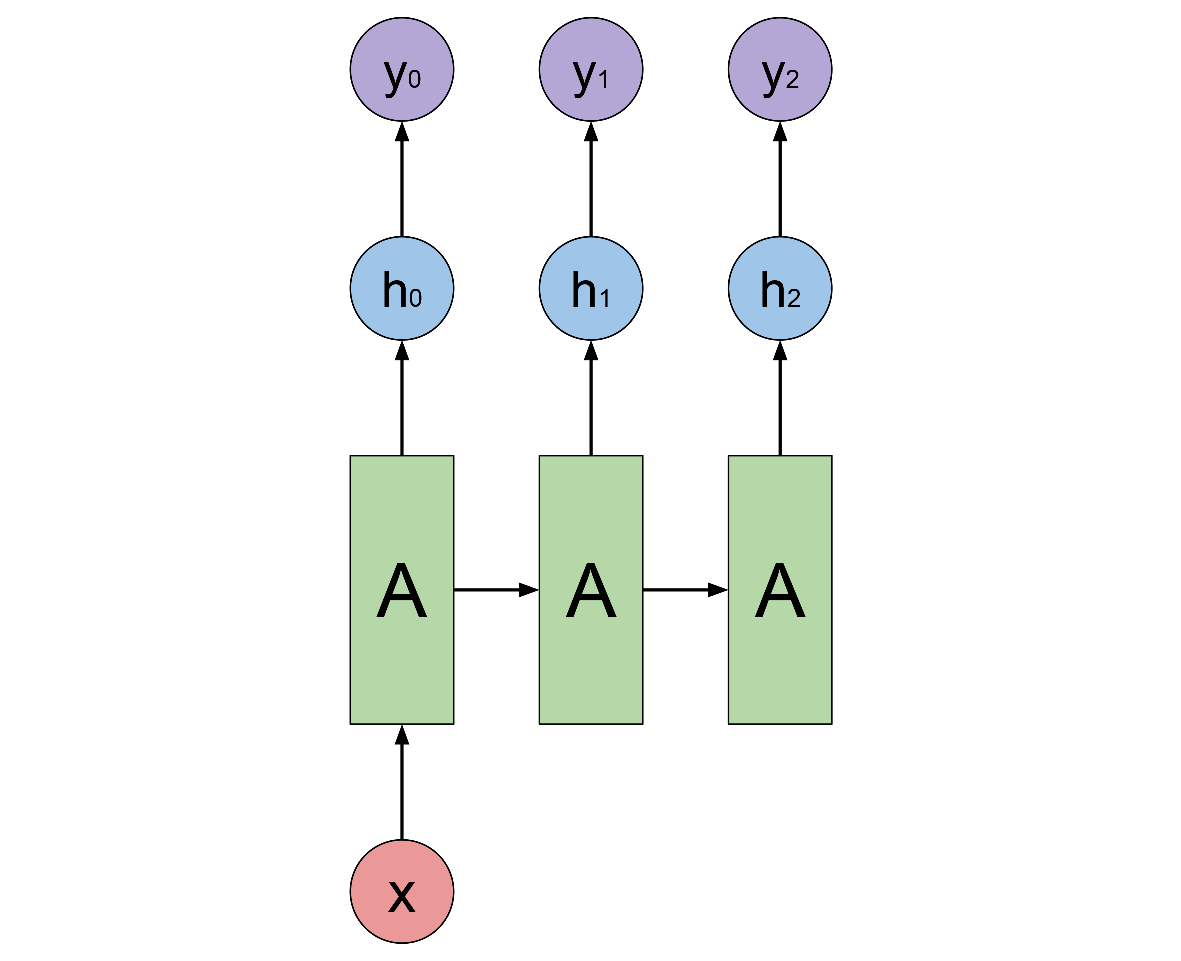
\includegraphics[height=0.2\textwidth]{images/one_to_many.pdf}\end{center} \\
% \hline
% This is some text & \begin{center}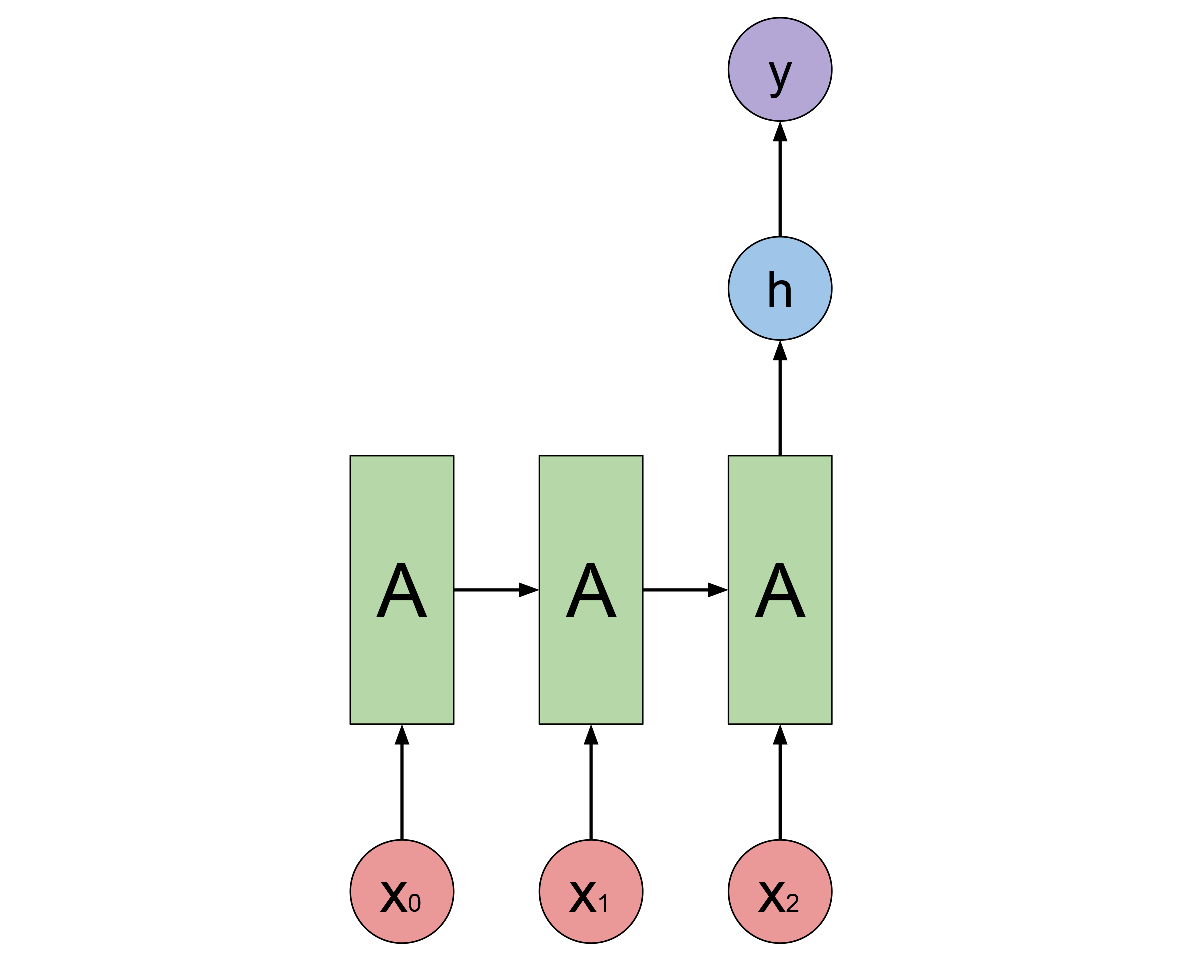
\includegraphics[height=0.2\textwidth]{images/many_to_one.pdf}\end{center} & This is some text & \begin{center}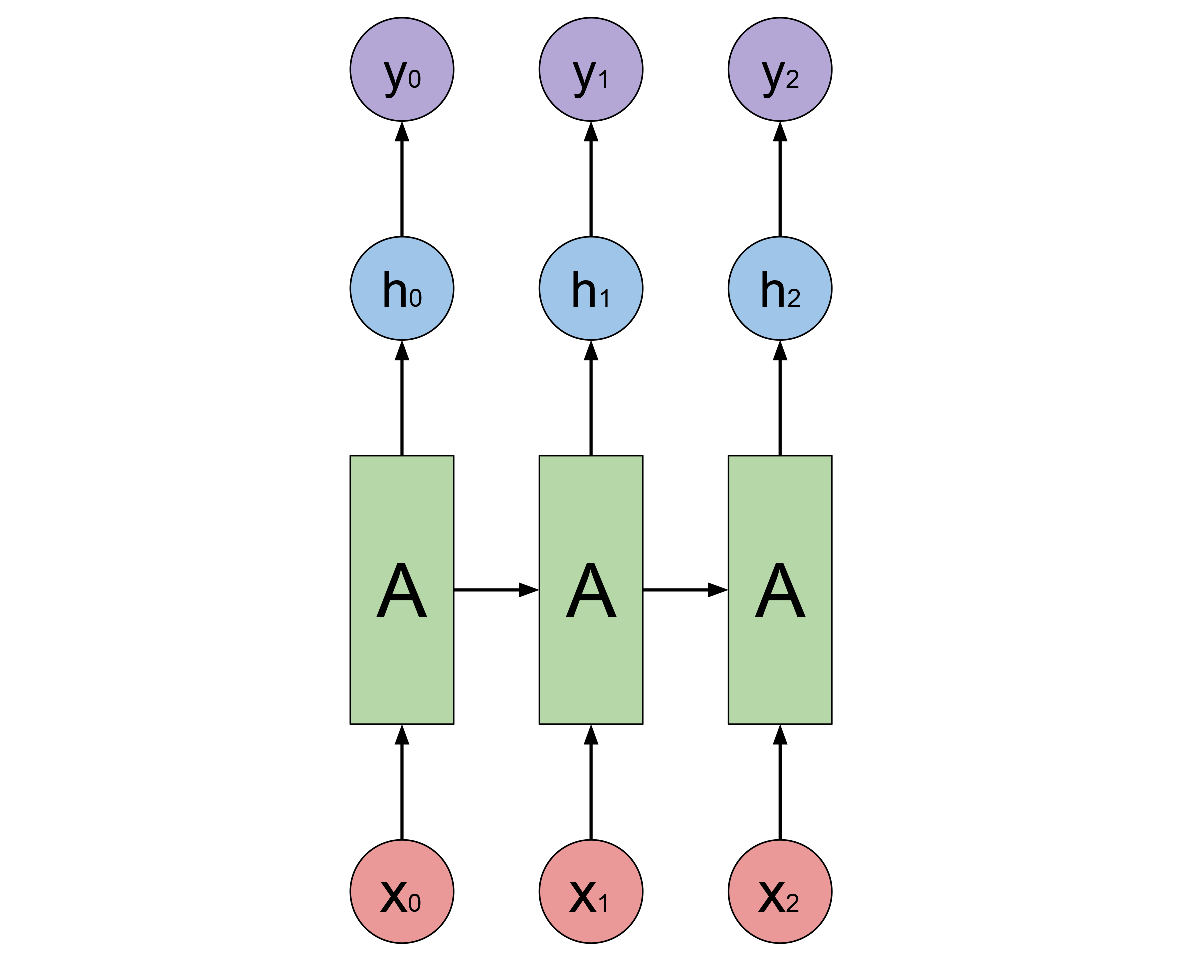
\includegraphics[height=0.2\textwidth]{images/many_to_many.pdf}\end{center} \\
% \hline
% This is some text & \begin{center}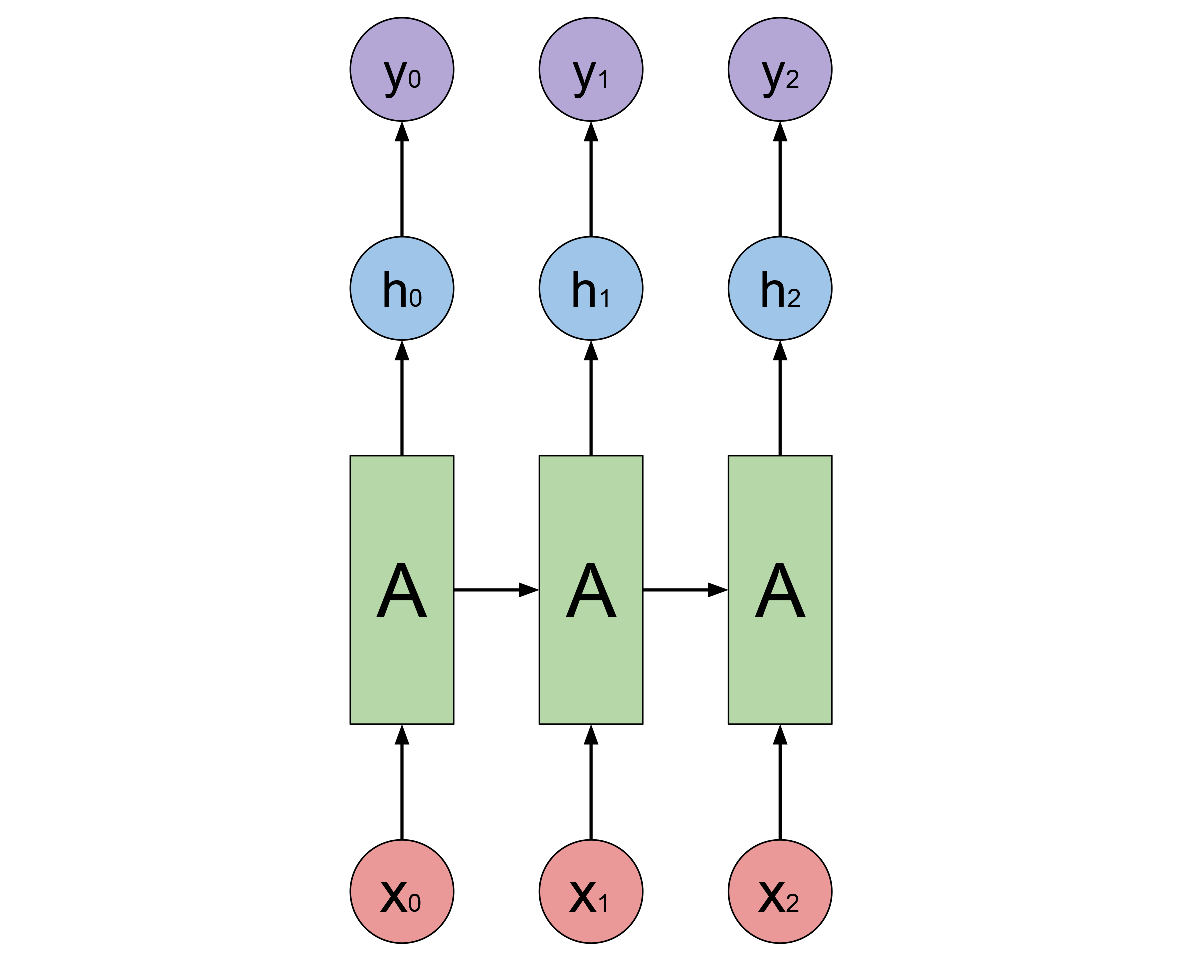
\includegraphics[height=0.2\textwidth]{images/many_to_many.pdf}\end{center} & & \\
% \hline
% \end{tabular}
% \label{tab:gt}
% \end{table}

% \begin{itemize}
%     \item One-to-One if $l_x = l_y = 1$, this is a traditional neural network;
%     \item One-to-Many if $l_x = 1, l_y > 1$, this is the case for sequence generation;
%     \item Many-to-One if $l_x > 1, l_y = 1$, for sequence classification;
%     \item Many-to-Many if $l_x = l_y > 1$, for sequence labeling;
%     \item Many-to-Many if $l_x \neq l_y, l_x > 1, l_y > 1$, for sequence to sequence tasks.
% \end{itemize}

We can also have bidirectional RNN~\citep{Schuster1997birnn} (biRNN), which is composed of two RNNs, one looks at the sequence starting from the end while the other from the beginning as usual. The output at each step of a bidirectional RNN is the concatenation of the hidden states for that time step. In a biRNN we have a left-to-right hidden state (or forward state) $\overrightarrow{h_t} = RNN(x_t, \overrightarrow{h}_{t-1})$, a right-to-left one (or backward state) $\overleftarrow{h_t} = RNN(x_t, \overleftarrow{h}_{t-1})$, and the output hidden state $h_t$ is defined as the concatenation of the directional hidden layers: $h_t = [\overrightarrow{h_t}, \overleftarrow{h_t}]$. The advantage of having bidirectional information is quite clear, the model is able to represent also future information, so the current decision is affected by both past and future.

Recurrent networks have various advantages over traditional networks. These include the ability to process sequences of any length, the size of the model does not increase with the size of the input, and the most important, the computation takes into consideration historical information that should allow RNNs to learn long-term dependencies. Unfortunately, they also have some drawbacks; they are computationally more intensive. Moreover, even if they can work with a sequence of any length and pass information through time, this information transfer starts to become less effective for longer sequences, which means they struggle to model long-term dependencies. That is caused by the vanishing/explosion of the gradient, a significant issue in vanilla RNN. 

The vanishing gradient problem was first studied by~\cite{Hochreiter:91} and ~\cite{bengio1994vanishing}. The problem occurs when we try to train a neural network model using gradient-based optimisation techniques, the backpropagation of the loss function with respect to the weights tends to vanish. This is a consequence of what happens during forward propagation; the hidden state is multiplied several times with the weight matrix, once per time step. So, during backpropagation, this leads to the gradients being multiplied by the same values many times, causing the values to either explode, i.e. grow extremely large or vanish, i.e. become very small, making the model unable to learn. In RNNs this translates to that is very tough to allow the error to flow from the later in time inputs to the ones at the beginning, thus creating difficulties to train the early stages of the RNN and reducing the ability to learn long-term dependencies due to insufficient weight changes.

% \begin{equation}
% \begin{split}
%     h_t & = tanh(W_{h} * h_{t-1} + W_x * x_t) \\
%     y_t & = W_y * h_t
% \end{split}
% \end{equation}

% \begin{figure*}[ht!]
%     \centering
%     \begin{subfigure}[t]{0.3\textwidth}
%         \centering
%         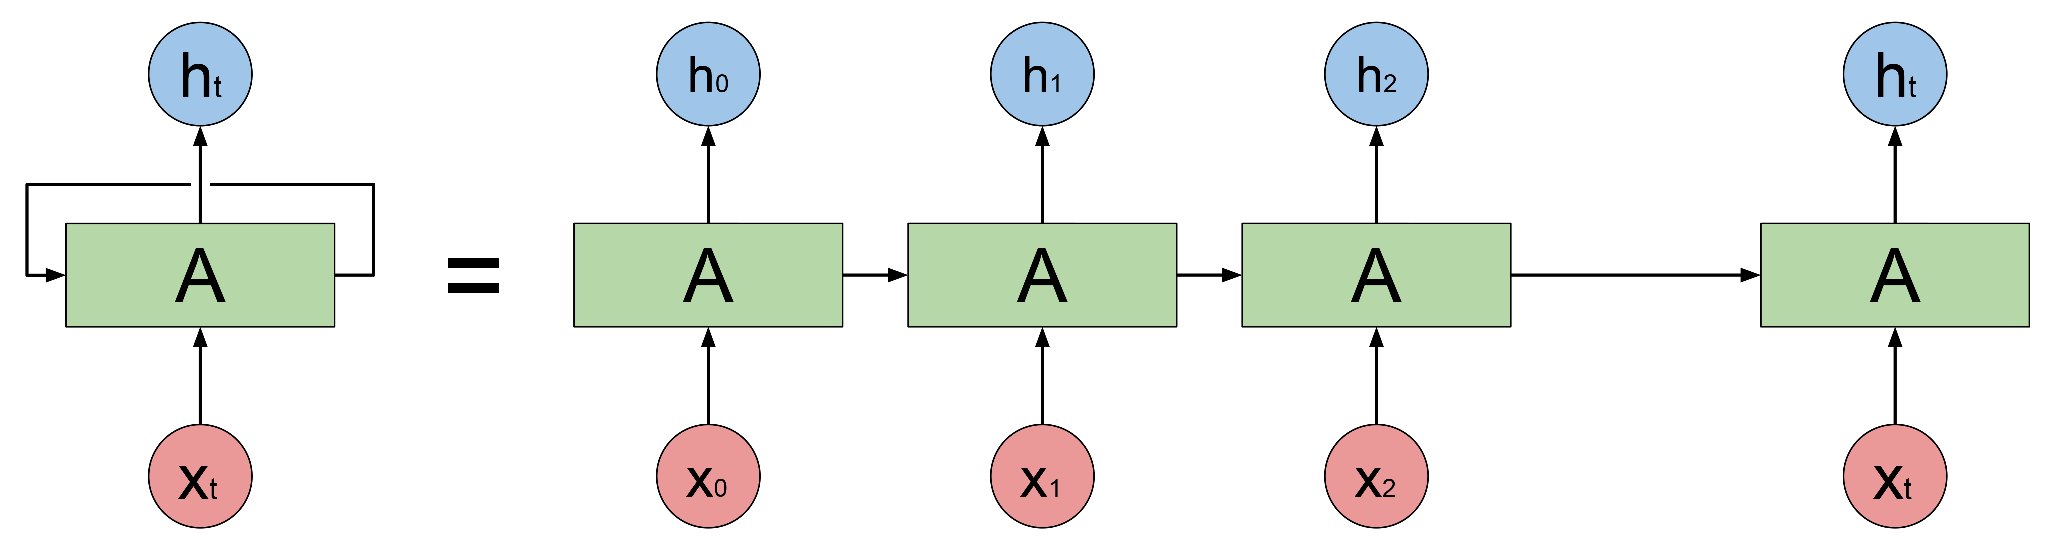
\includegraphics[width=0.7\textwidth]{images/RNN.png}
%         \caption{}
%         \label{subfig:rnn}
%     \end{subfigure}%
%     ~ 
%     \begin{subfigure}[t]{0.7\textwidth}
%         \centering
%         \includegraphics[width=\textwidth]{images/RNN-unrolled_only.png}
%         \caption{}
%         \label{subfig:rnn_unrolled}

%     \end{subfigure}
%     \caption{Different views of a recurrent neural network. In Figure~\ref{subfig:rnn} we have the compact view. Figure~\ref{subfig:rnn_unrolled} shows the same architecture but unrolled. Image credit: Christopher Olah}
%     \label{fig:rnn}
% \end{figure*} 


\subsection{Long Short Term Memory}
\label{sec:lstm}

\begin{figure}[]
    \centering
    \begin{subfigure}[t]{0.5\textwidth}
        \centering
        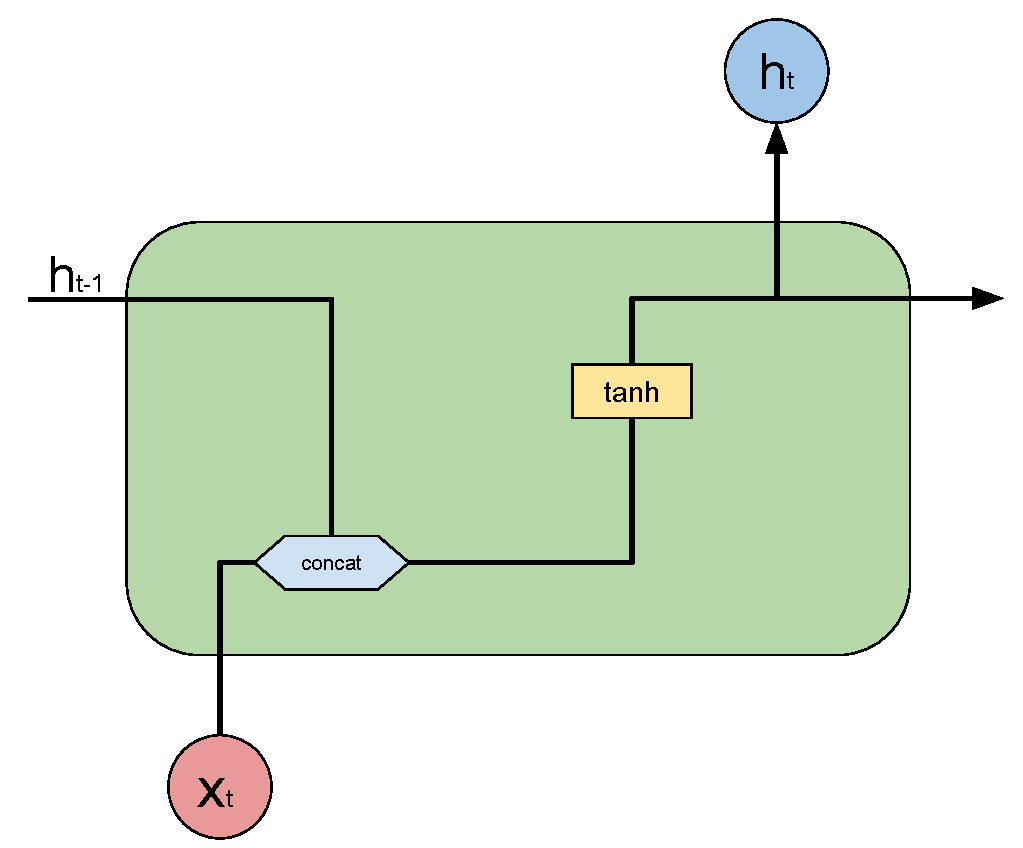
\includegraphics[width=\textwidth]{images/RNN_cell_simple.pdf}
        \caption{Vanilla RNN cell}
        \label{subfig:rnn_cell}

    \end{subfigure}%
    ~ 
    \begin{subfigure}[t]{0.5\textwidth}
        \centering
        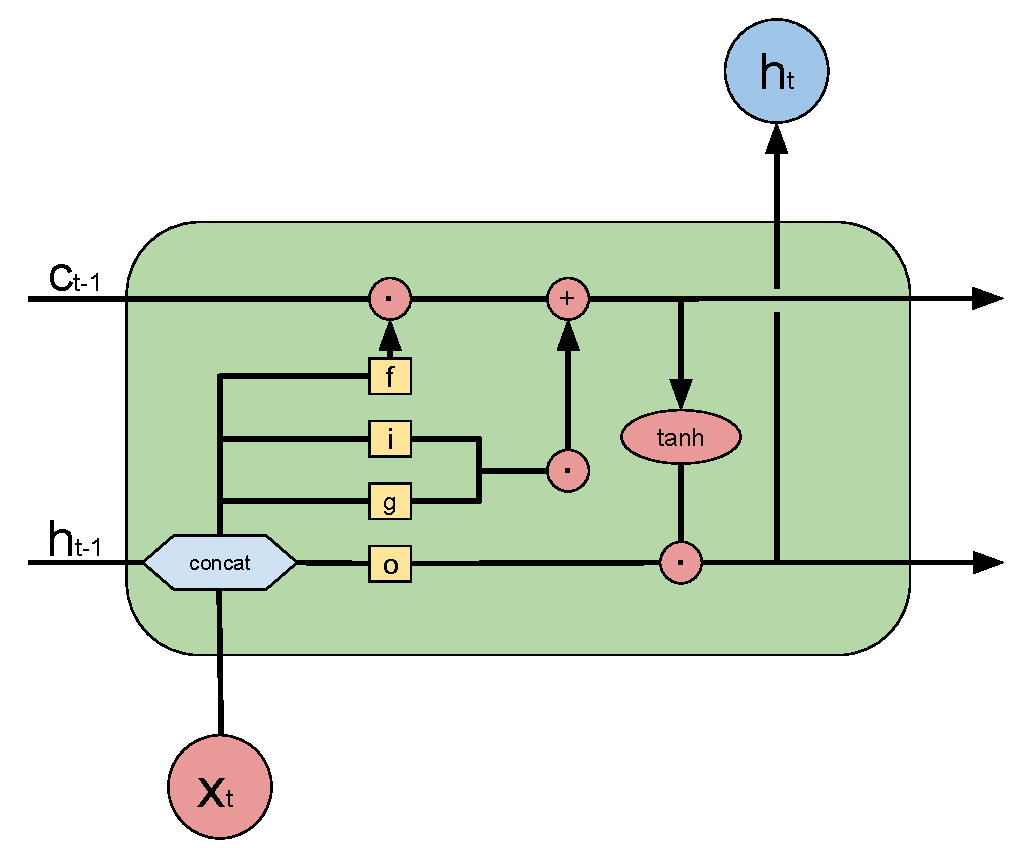
\includegraphics[width=\textwidth]{images/LSTM_cell_simple.pdf}
        \caption{LSTM cell}
        \label{subfig:lstm_cell}

    \end{subfigure}
    \caption{Different types of cells. Red circles are for point-wise operations, in yellow we have neural networks.} % activation functions (these can be seen as neural network, where the weights are in W, and they use different parts of W). } % The blue circle is the dot product, and the stack operation creates a n-dimensional vector with n as the number of input elements.}
    \label{fig:cells}
\end{figure} 

\paragraph{}
Long Short Term Memory networks (LSTM) are an improved version of RNN  that introduces mechanisms to decide what should be ``remembered'' and ``forgotten''. Proposed by~\cite{hochreiter1997long}, LSTMs are a solution to the long-term dependencies issue in vanilla RNN and the vanishing of the gradient. LSTMs mitigate the problem by having a more complex cell that contains two hidden states. The first one is $h_t$ and is similar to the one in RNNs, the other is $C_t$, the cell state, which is the core of a LSTM cell. The cell state is modified using the gates, which are neural networks acting on the information of the cell state and the hidden state. In Figure~\ref{fig:cells} we can see how the information flows and interact with the different gates, these are:

\begin{itemize}
    \item Forget gate layer ($f$): acts on what and how much to forget from the previous time step. It is computed using a neural network with a sigmoid $\sigma$ activation function. The output of the network is between 0 and 1, since the output will be multiplied element-wise 0 means forget all, and 1 remember all. $f_t = \sigma(W_f * [h_{t-1}, x_t])$;
    \item Input gate layer ($i$): this gate decides which information to write to the cell state. It is a sigmoid layer: $i_t = \sigma(W_i * [h_{t-1}, x_t])$, and works in combination with the gate layer; 
    \item Gate gate layer ($g$): decides how much to write to the cell state. It is a $\tanh$ layer, $g_t = \sigma(W_g * [h_{t-1}, x_t])$. The output is the multiplied by the input gate output to create a new candidate state cell that will be summed with the value of the previous cell state after the forget step. The new cell state is  $c_t & = f_t \odot c_{t-1} + i_t \odot g_t$;
    \item Output gate layer ($o$): this layer is responsible of how much of the cell state to reveal through the hidden state. This is done using a sigmoid layer which decides the parts of the cell state that will be shown in the output, formally $o_t = \sigma(W_o * [h_{t-1}, x_t])$. Then, we put the cell state through $\tanh$ (to push the values to be between −1 and 1) and multiply it by the output of the output layer, so that we only expose the parts we decided to. Formally, the hidden state will be $h_t & = o_t \odot \tanh(c_t)$.
    
\end{itemize}


% The previous equations can be wrote more compactly as show in Equation~\ref{eq:lstm}. We have $W \in \mathbb{R}^4$, where each element is a matrix of weights for the different layers of the cell. The hidden layer $h_t$ and the input $x_t$ are both vectors. And $\sigma$, $tahn$ are the activation functions. 

% \begin{equation}
% \begin{split}
%          W & = [W_i, W_f, W_o, W_g] \\ 
%          \begin{bmatrix}
%           i \\
%           f \\
%           o \\
%           g   
%         \end{bmatrix} & =         \begin{bmatrix}
%           \sigma \\
%           \sigma \\
%           \sigma \\
%           \tanh
%          \end{bmatrix}  W   \left[ h_{t-1}, x_t\right]\\
%          c_t & = f \odot c_{t-1} + i \odot g \\
%          h_t & = o \odot \tanh(c_t) \\
% \end{split}
% \label{eq:lstm}
% \end{equation}

This is the general LSTM; however there are many variants of LSTMs, which perform slightly better or worse depending on the task. A more detailed work on how each variant perform is ``LSTM: A Search Space Odyssey'' by~\citet{greff2017lstm}.


\subsection{Attention mechanism}

\begin{figure}[t]
        \centering
        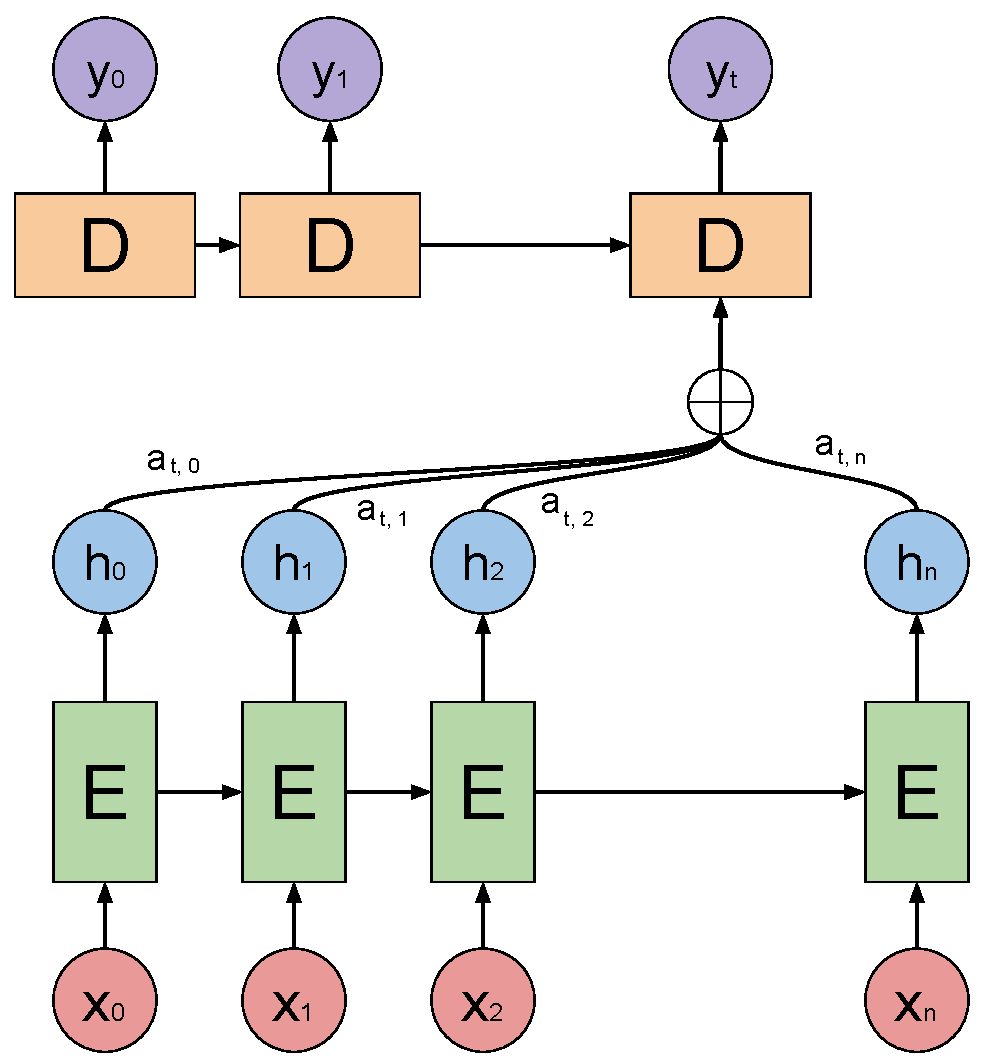
\includegraphics[width=0.5\textwidth]{images/Attention.pdf}
        \caption{Attention mechanism. The encoder $E$ hidden states are weighted via $a_{i, j}$, summed, and used as input to the decoder $D$ to produce the output at step $t$.}
        \label{fig:attention}
\end{figure}%

\paragraph{}
A very popular RNN architecture is the sequence to sequence, or encoder-decoder ~\citep{cho-etal-2014-learning,sutskever2014sequence}. This framework is used in neural machine translation, text summarization, question answering, and many more. 
% \begin{wrapfigure}{r}{0.5\textwidth}
%         \centering
%         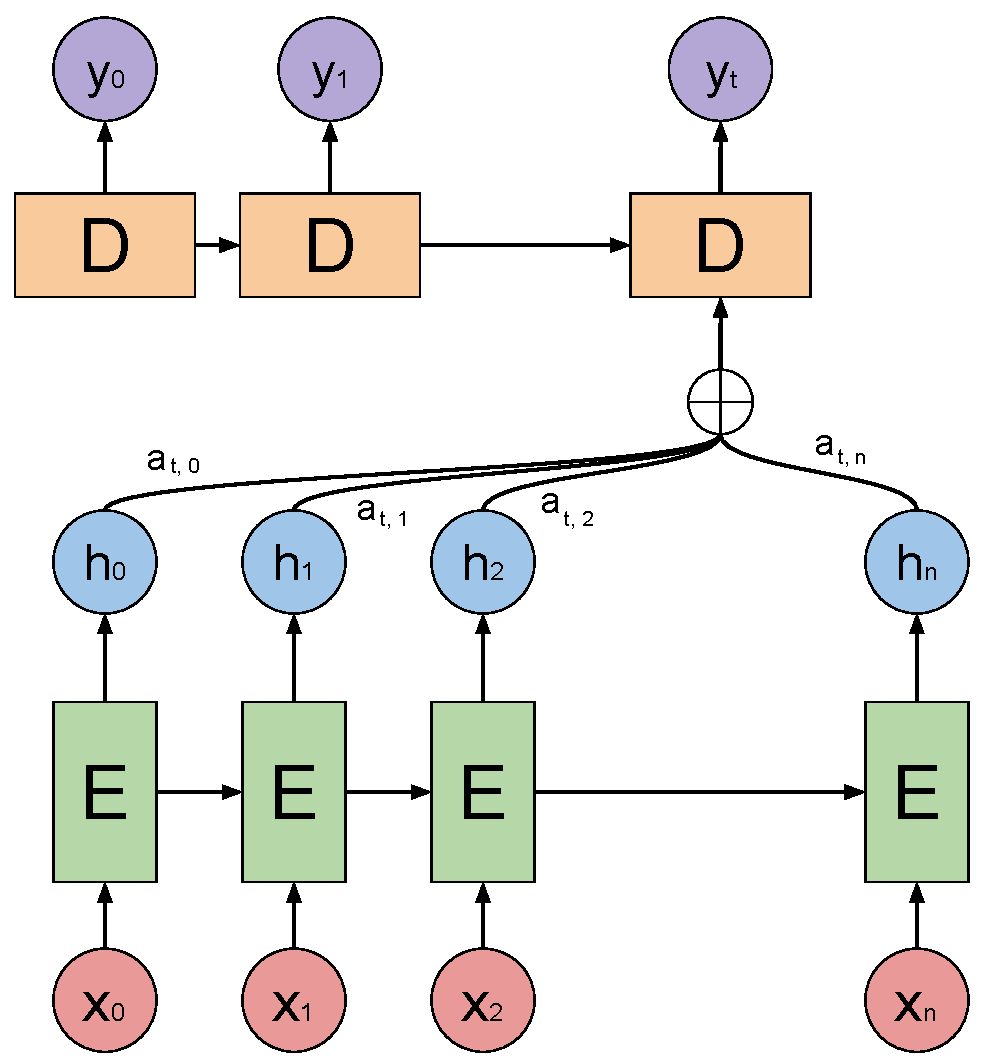
\includegraphics[width=0.5\textwidth]{images/Attention.pdf}
%         \caption{Attention mechanism. The encoder $E$ hidden states are used as input to the decoder $D$ to produce the output of at step $t$.}
%         \label{fig:attention}
% \end{wrapfigure}%

A sequence to sequence model is composed by an encoder, which takes the input sequence and compresses it into a context vector which will be used to start the decoder which predicts a output sequence.  A significant and clear disadvantage of a fixed-length context vector design is as the input sequence get compressed into a single vector, and as this sequence gets longer and longer, more memory is required to store past information. As a result, the network performs poorly o longer sequences~\citep{cho-etal-2014-properties}. A solution to this problem was proposed by~\cite{bahdanau2014neural}, which defines an attention mechanism for the decoder. Instead of just relying on the previous hidden state, the decoder with attention can use the information from all the input sequence by looking at the encoder hidden state at each time step, and combine this information to produce the output.

\paragraph{Encoder:} Given a sequence of vectors $\textbf{x} = (x_1, \dots, x_n)$, an RNN takes this sequence and produces a context vector $c$:

\begin{equation}
    \begin{split}
        h_t & = f(x_t, h_{t-1})\\
        c & = q(\{h_1, \dots, h_n\}) 
    \end{split}
\end{equation}

where $h_t$ is the hidden state at time $t$, and $f$ and $q$ are nonlinear functions. Some example of $f$ and $g$ include: LTSMs for $f$, and return the last hidden state for $g$. This part is the same with or without attention mechanism.


\paragraph{Decoder:}

\paragraph{Decoder with Attention:}

Illustrated in Figure~\ref{fig:attention}

\subsection{Transformer}

\section{Word Representation}
\label{sec:word_embedding}
\paragraph{}
Word representation is an elemental part of most Natural Language Processing (NLP) tasks. The understanding of text is mainly derived by transforming text to usable computational representations, these include graphs, trees, or vectors on which will the focus.   In general, it has been found to be beneficial to represent words or documents as vectors, which have an appealing, intuitive interpretation, and they capture hidden information concerning a language, like word analogies or semantic. 
%A word representation is a mathematical object associated with each word, often a vector.

% Based on the literature \citep{turian2010word, schnabel2015embeddings},  \cite{almeida2019word} define word embeddings as a e dense, distributed, fixed-length word vectors, built using word co-occurrence statistics as per the distributional hypothesis

There are various methods to induce word representation:

\begin{itemize}[itemsep = 0.1em]
\item Distributional word representation: are based on co-occurrence context and on the distributional hypothesis:  ``\textit{linguistic items with similar distributions have similar meanings}'', hence the similarity is expressed in terms of the similarity of the distribution. Some common representation techniques include Latent Semantic Analysis~\citep{deerwester1990indexing} and Latent Dirichlet Allocation~\citep{bei2003lda, das-etal-2015-gaussian}. An important example is the work of \citet{pennington2014glove} which propose a competitive set of pre-trained word representations, his work signals that word representation had reached the main stream.

\item Distributed representation: are compact, dense and low dimensional representation, where each dimension of the embedding represents a latent feature of the word, hopefully capturing useful syntactic and semantic properties. A distributed representation is compact, in the sense that it can represent an exponential number of clusters in the number of dimensions. Some examples include the work of \citet{Collobert2008} which for the first time demonstrated the utility of word embeddings for downstream tasks and their proposed neural network architecture forms the foundation for many current approaches, and the Word2Vec framework proposed by \citet{mikolov2013distributed} which popularized word embeddings.
\end{itemize}

In the work ``\textit{Word representations: A simple and general method for semi-supervised learning}'', \citet{turian2010word} define as ``\textit{word embeddings}'' only the distributed representation, but over time this distinction is not enforced and is common to refer to all vector word representations as word embeddings.


\paragraph{}
Another essential part of NLP is the study of language models. A language model is a statistical model of language usage. It consists mainly of predicting the next word given some previous words. A language model learns the probability of word occurrence based on examples of text. Simpler models may look at a context of a short sequence of words, whereas larger models may work at the level of sentences or paragraphs.

More formally, the goal of a statistical language model is to learn the probability $P(x_1, \dots, x_m)$ for a sequence of tokens $x_1, \dots, x_m$. We can compute this via the chain rule of probability:

\begin{equation}
P\left(w_{1}, \ldots, w_{m}\right)=\prod_{i=1}^{m} P\left(w_{i} | w_{1}, \dots, w_{i-1}\right)
\end{equation}

Because the number of words that precede a word varies, and because it is difficult to compute $P(w_i | w_1,\dots, w_{i-1})$ with $i$ large, we typically condition the probability of a word on a window of n previous words ($n$-grams): 


\begin{equation}
P\left(w_{1}, \ldots, w_{m}\right) \approx \prod_{i=1}^{m} P\left(w_{i} | w_{i-n}, \dots, w_{i-1}\right)
\end{equation}

This approach doesn't generalize to new sequences, unless using some tricks like~\citet{katz1987probablm} did where he computes small $n$-grams, generally $n=3$, and then generalizes to unseen sequences by producing new ones using overlapping n-grams of length up to $n$. However, this solution does not generalize to sequences longer than $n$, which has to be small, and also does not take in consideration the similarities of words. Moreover, statistical language models suffer from the problem known as curse of dimensionality that appears when the vocabulary size increases. For example, computing the joint probability of 10 consecutive words having a vocabulary size of 100k there are $100000^{10} - 1 = 10^{50} - 1$ free parameters. 

\citet{bengio2003nnlm} develop a solution for the course of dimensionality of statistical language models by proposing the first large-scale language model based on neural networks, referred to as Neural Network Language Models (NNLMs). In their work \citet{bengio2003nnlm} bring together language modeling and word embeddings by \begin {enumerate*} [1) ]%
\item associating each word in the vocabulary with a distributed word vector called ``\textit{feature vector}'' \item express the joint probability function of word sequences in terms of the feature vectors of these words in the sequence; \item learn simultaneously the word feature vector and the parameters of the probability function.
\end {enumerate*} This new representation also generalizes to longer sequences and is able to learn similarities between words. \citet{bengio2003nnlm} conclude their work by suggesting the use of Recurrent Neural Networks (RNN) to take advantage of temporal structures and also consider longer sequences like entire paragraphs.

A few years later, \citet{Mikolov2010RecurrentNN} propose a neural language model based on RNN, they use a vanilla RNN~\citep{elman1990finding} to show how language models based on recurrent networks are significantly better that previous solution. They perform experiments on various speech recognition task, and achieve better results even when training using lower amount of data.

This work and the one of \cite{bengio2003nnlm} were followed by many other word embeddings solutions that build upon their methods, in particular current state of the art use RNN, or improved versions like Long Short Term Memory networks~\citep{hochreiter1997long}. We will now present in more detail some of these works using the following architectures: GloVe~\citep{pennington2014glove}, ELMo~\citep{peters2018elmo},and the two we used in our experiments, BERT~\citep{devlin2018bert} and fastText~\citep{bojanowski2016enriching}.


 %Move fT, and BERT in MODEL

\subsection{fastText}
\subsection{BERT}


\subsection{Multilingual Word Representation}

\section{Transfer Learning}
\label{sec:transfer_learning}
\subsection{Cross-lingual Learning}
\subsection{Multi-task Learning}
 
\section{Zero-Shot, One-Shot and Few Shot Learning} 
\label{sec:zero_learning}

\chapter{State of the Art} % Relation Extraction? | Natural Language Understanding
\label{chpt:3}
\section{Relation Extraction}
\subsection{Zero-Shot Relation Extraction}
\subsection{Multilingual Relation Extraction}

\section{Machine Comprehension}
\subsection{BiDAF}
% \subsection{NAMANDA}
\chapter{State-of-the-Art} % Relation Extraction? | Natural Language Understanding
\label{chpt:3}
\paragraph{}
In this Chapter we will present the literature for the relation extraction task (Section~\ref{sec:sota_re}) and for the machine reading comprehension (Section~\ref{sec:sota_mc}). Each section will give a definition of the task, and present an overview of the solutions adopted to solve the task. We will also show how these solution are adopted in a multilingual setup, and for the relation extraction task, present some literature on the zero-shot scenario.   


\section{Relation Extraction}
\label{sec:sota_re}
\paragraph{}
In the following sections we will present the relation extraction task. We will start with a definition, we will present some approaches to solve the task, with examples for both multilingual and zero-shot learning scenarios.

\subsection{Introduction}
Many applications in information extraction, natural language understanding, information retrieval require an understanding of the semantic relations between entities. This information is usually contained in unstructured data like blogs, news articles, and so on.  Relation extraction aims at making this information usable by other system by extracting the relations contained in unstructured documents and make is available in knowledge bases.

A relation is defined in the form of $r(e_1, e_2, ..., e_n)$ where the $e_i$ are entities in a relation $r$ within document $D$. We will focus on relations with only 2 entities, and refer to the entity pairs and relation as triples, as is common also the use of the following notation $(e_1, r, e_2)$. Since our dataset is built from Wikipedia and Wikidata, throughout this work, we use the term property interchangeably with relation. Given human readable text, relation extraction is the task of identifying instances of relations $r(e_1,e_2)$. For example, in the sentence: ``Elon Musk is the CEO of both Tesla and SpaceX", a system should be able to extract the relations \textit{chief\_executive\_officer({Elon Musk}, Tesla)}, and \textit{chief\_executive\_officer(Elon Musk, SpaceX)}. 

Simple relation extraction can be achieved using rules, however, rule-based systems require a deep knowledge of the domain and high human annotation time. In the supervised setting~\citep{bach2007review}, depending on the nature of input to the classifier, approaches are further divided into feature based methods and kernel methods. For the feature based systems both the semantic and syntactic features are used as input to the classifier in the form of a feature vector. In~\citep{Kambhatla2004extraction} they use maximum entropy models, or ~\citep{zhao-grishman-2005-extracting, zhou-etal-2005-exploring} uses SVMs trained on the features with different kernel types.

These solution however still rely on human domain knowledge for the definition of the features, this can be solved using end-to-end solutions like in~\citep{miwa-bansal-2016-end, pawar-etal-2017-end}. In an end-to-end relation extraction the system has to identifies both the entities, their type and the relation holding between them, if any.~\cite{miwa-bansal-2016-end} uses a biLSTM on both the word sequences, and tree structures. In~\cite{pawar-etal-2017-end} they train a joint model to predict the boundaries, the type of the entities and the relation between them. 

The clear drawback of supervised methods is the need of training data: data labeling is expensive, and there is often a mismatch between the training data and the data the system will be applied to. A solution to this problem has been proposed in~\citep{plank-moschitti-2013-embedding}. They use domain adaptation techniques, and build a model that uses syntactic tree kernels enriched by lexical semantic.

An alternative type of relation extraction is Open Relation Extraction (Open RE)~\citep{banko2007openre, banko-etzioni-2008-tradeoffs}. Instead of having a fixed set of relations, Open RE aims at extracting relational triples from an open-domain corpus.  In~\citep{banko2007openre} in addition to the introduction of the Open RE task, they propose TextRunner, a large scale relation extraction tool on open domains. TextRunner uses a self-learner to automatically label if there exists a relation between the extracted entities in the text. The examples, both positive and negative are used to train a Naive Bayes classifier. The use of patterns between mentions as relations removes the requirement of supervision and has high flexibility, however it lacks generalization. A solution to the generalization issue is by clustering the surface form of words with similar meaning~\citep{yao-etal-2011-structured}.

\cite{riedel2013relation} remove the need of a defined schema by using Universal Schemas, the union of all involved schemas (surface form predicate as in~\citep{banko2007openre}, and relations in the schema of pre-existing databases). They model the problem as a probability of a relation holding between two entities, this allows them to use solutions from collaborative filtering. In particular they perform matrix factorization on the matrix with entity tuples are rows, and the columns are the union of the surface forms and the DB relations. More formally, they model the probability of two entity $t = (e_1, e_2)$ being in relation $r$ by using an exponential function parametrized by a natural parameter $\theta_{r, t}$:

\begin{equation}
    P(y_{r, t} = 1 | \theta_{r, t}) = \frac{1}{1+exp(-\theta_{r,t})}
\end{equation}

the parameter $\theta_{r,t}$ can be computed in different ways (e.g. the the dot product of the latent feature representation of the relation and the tuple).

By defining the matrix using the entity pairs, we can only predict relations between entity seen at train time. \cite{verga-mccallum-2016-row} propose a row-less universal schema. Instead of encoding each pair explicitly, they use aggregation functions over the over the observed instances. The embedding of the pairs can be seen as a summarization of all relation types the entities were seen in.

\subsection{Multilingual Relation Extraction}
\paragraph{}
Earlier works investigating multilingual relation extraction have been few and far between. In \cite{faruqui2015multilingual} they perform multilingual RE by translating the sentences in English and the run a Open RE system. This solution is simple and relies only on the availability of a translator from the target language to English. \cite{verga2015multilingual} uses universal schemas on top of multilingual embeddings to extract relations in a target language without  using  training  data in the target language. 

\cite{lin-etal-2017-neural} proposes one of the first neural multilingual solution for RE. They use use an dataset of English articles from Wikipedia, and Chines articles from Baidu Baike (a Chinese-language online encyclopedia). The articles were aligned annotated using Wikidata. They use a sequence-to-sequence model with both a cross-lingual and mono-lingual attention. The cross-lingual attention helps with sentences with strong consistency across the languages.   

\subsection{Zero-shot Relation Extraction}
\paragraph{}
\cite{levy2017zero} proposes a new approach to relation extraction that allows zero-shot learning. They propose a novel approach towards achieving this generalization by transforming relations into natural language question templates. This means that we can translate a relation \textit{born\_in(X, Y)} into the question \textit{``When was X born?"}, or \textit{``In what year was X born?"} . Reframing RE as a question answering problem, allows the use of reading comprehension models. In particular, they use BiDAF~\citep{seo2016bidirectional}, a machine comprehension model that uses BiLSTM and attention mechanism to find the answer of a question given a context (more detailed description in Section~\ref{sec:bidaf}). The reading comprehension model is trained using the question, answer, and context examples where the \textit{X} slot is filled with an entity and the \textit{Y} slot is either an answer, if the answer is present in the context, or \texttt{NIL}. The model is then able to extract relation instances from raw text, even for relations which has not been seen during training, enabling zero-shot relation extraction.

Another solution has been proposed by \cite{goldstein2018zero}. They achieve zero-shot relation extraction using word embeddings. They  construct triples $(A, r, B)$, where $A, B$ are matrices where each column vector represents an entity. Entities in the same column but in the other matrix are in relation $r$. The triples are used as a starting point to find other entities that are in the same relation $r$. $A, B$ are obtained by performing bootstrapping using a seed entity on the word embedding vector space. After the small set of entities was found, they are used to generalize to new ones. This is achieved by finding the most common features between all possible pairs on entities, and reducing the space to only these features enabling to find other entities in relation using the distance of the points. A method based on embedding vector space brings different advantages like the ability to find duplicate relation (e.g. misspelled relations), and the ability to correct the model by using the new added information. 
 

\section{Machine Reading Comprehension}
\label{sec:sota_mc}
\paragraph{}
In the next sections we will talk about the Machine Reading Comprehension task. We will present the literature and take a closer look at a model, to better understand how these models work.

\subsection{Introduction}
\paragraph{}
Childrens' ability to read is evaluated by giving them reading comprehension tests. These test typically consist of a short paragraph followed by questions. The questions are designed in such a way that to answer correctly the reader has to understand the content of the text. Similar tests are also used to measure machine's ability to understand documents. Machine Reading Comprehension (MRC) has gained a lot of interest in the last years with the introduction of sequence-to-sequence models, and datasets like SQuAD~\citep{rajpurkar2016squad, rajpurkar-etal-2018-know}. 

The reading comprehension task easily conforms to a formulation as a supervised learning problem. Specifically, given a context document $c$,  a query $q$ relating to that document, and the answer $a$ to that query,  goal is to estimate the conditional probability $P(a|c, q)$. Depending on the type of the question an the answer, reading comprehension can be of four types:

\begin{itemize}[- ,noitemsep]
    \item Cloze-style: same as in the Cloze task~\citep{taylor1953cloze}, the question contains placeholder that the system has to fill;
    \item Multi-choice: the answer can be only one of multiple choices;
    \item Span-prediction: the machine needs to find the correct answer in the passage by predicting the spans. This category is also referred to as extractive question answering;
    \item Free-form: the answer is human-generated, so there are some problems with the evaluation.
\end{itemize}

Traditional systems rely on solutions from information extraction, by detecting predicate argument triples that can later be queried as a relational database~\citep{poon-etal-2010-machine} or pattern matching, and use statistical and mathematical methods to perform similarity between the question and the answer to find the correct answer. For example, in~\citep{riloff-thelen-2000-rule} they propose QUARC (QUestion Answering for Reading Comprehension) a rule-based system that uses lexical and semantic heuristics to look for an indication that a sentence contains the answer to a question. Each type of \textit{``Wh"} question looks for different types of answers, so QUARC uses different sets of rules for each question type. These solutions are not actually understanding a given passage, so they lack the reasoning we would expect from a reading comprehension model.

Recent solution are based on neural networks, and popular architectures like the sequence-to-sequence model. These methods all share a common structure as described in~\citep{qiu2019survey}. The passage and the answer both pass to an embed layer,an encoding one, then the encodings are used together by the match layer, which outputs to the answer layer. The layers role are:

\begin{itemize}[- ,noitemsep]
    \item Embed layer: this layer converts the words into their representations as seen in Section~\ref{sec:word_embedding};
    \item Encoding layer: produces a representation of the input, this can be produced using LSTMs, or other sequence encoding models;
    \item Match layer: captures the interaction between the context and the question, and produces a query-aware context representation;
    \item Answer layer: it predicts the correct answer, the answer can be of different types as mentioned before.
\end{itemize}

The use of neural networks solutions, and sequence-to-sequence models for reading comprehension was popularized by~\citep{hermann2015teaching, weston2015memory}. \cite{weston2015memory} proposes a new model architecture called Memory Network. Memory Network, which is a framework with four components \begin {enumerate*} [1) ]
\item a component that transforms the input into the internal representation 
\item one that changes the memory states using the input, and the memory
\item the component that generates the the output features based on the memory, and the input
\item the last component that decodes the features to predict the output.
\end {enumerate*} 
The component can be any model (SVM, NN, etc.). They also propose a Memory Neural Network (MemNN) for the reading comprehension task. 

\cite{hermann2015teaching} uses RNNs with attention mechanism, and proposes two models, the Attentive Reader and the Impatient Reader. The first one encodes the query using bidirectional LSTM and concatenates the results to get the representation of the query. The representation of the document is formed by a weighted sum of the BiLSTM outputs at each time step. The model is completed with the definition of the joint document and query embedding using a nonlinear combination. The Impatient Reader improves the representation of the query by using a the same method employed for the document encoding. 

The two architectures proposed in~\citep{hermann2015teaching} are at the core of many other solutions \citep{kadlec-etal-2016-text, chen-etal-2016-thorough}. In ~\citep{cheng-etal-2016-long}, similarly to ~\citep{weston2015memory}, they increase the memory of the RNN. In particular they use a LSTM with a memory network instead of a single cell, the memory network enables adaptive memory usage and offers a way to weakly induce relations among tokens.



\subsection{BiDAF}
\label{sec:bidaf}
~\cite{levy2017zero} uses as their machine comprehension model BiDAF~\citep{seo2016bidirectional}. BiDAF (Bi-Directional Attention Flow) instead of using a single attention and/or focusing only on small portion of the text like previous solution did, it uses a multi-stage hierarchical process that represents the context and query at different levels of granularity and uses bidirectional attention flow mechanism to obtain a query-aware context representation. It follows the general architecture of all reading comprehensions model.

\subsubsection{Embed Layer}
Character embedding layer is responsible for mapping each word to a high dimensional vector space. BiDAF uses both character and word level embedding. Given a context $c =\{c_1, \dots, c_T\}$ and a query $q = \{q_1, \dots, q_J\}$, they are separately encoded using the concatenation of the character and word embedding vectors which are passed to a two layer Highway LSTMs~\citep{SrivastavaGS15highway}. The output are the representations of the context $C \in \mathbb{R}^{d\times M}$, and query $Q \in \mathbb{R}^{d\times M}$ at each step. These are passed to the encoding layer.

\subsubsection{Encoding Layer}
The encoding layer uses a BiLSTM to model the temporal interaction between words. The embeddings from the previous step are further encoded into $H \in \mathbb{R}^{2d\times N}$ for the context, and $U \in \mathbb{R}^{2d\times M}$ for the query. The next step is to find the interaction between them.


\subsubsection{Match Layer}
BiDAF match layer is further divided in two, the attention flow layer, and the modeling layer.
The former is responsible for finding the relevant information in the context regarding the query, and the vice versa. This is achieved by linking their information using attention. They compute two attention, a context-to-query and a query-to-context, they are a function of similarity matrix $S \in \mathbb{R}^{N\times M}$:

\begin{equation}
    S_{ij}= \alpha(H_{:u}, U_{:j})
\end{equation}

where $\alpha$ is a trainable scalar function that encodes the similarity between the vectors $H_{i:}$, and $U_{i:}$. The context-to-query attention is computed using the the attention weights  $a_t = softmax(S_{t:}) \in \mathbb{R}^{J}$ on the query words by $t$-th context word. The final attention matrix is $\tilde{U}$  contains the attended query vectors for the entire context, and $\tilde{U}_{:t}  = \sum_{j}a_{tj}U_{:j}$.

% \begin{equation}
%         \tilde{U}_{:t}  = \sum_{j}a_{tj}U_{:j} 
% \label{eq:c2q}
% \end{equation}

In the query-to-context attention the weights are $b_t = softmax({max}_{col}(S) \in \mathbb{R}^{T}$, and the attended context vector $\tilde{h} = \sum_{t}b_tH_{:t} \in \mathbb{R}^{2d}$ is the weighted sum of the most important words in the context. The final matrix $\tilde{H} \in \mathbb{R}^{2d\times T}$ is a $T$ times stack of $\tilde{h}$.

% $\tilde{U}$ is defined as weighted sum of the rowsoftmax of the matrix $S$ and the encoded context $U$, while the query-to-context $\tilde{U}$, the weights are computed as a $max$ over the columns with softmax, then a weighted sum is performed to obtain  



% \begin{equation}
%     \begin{split}
%         \tilde{H} = [\tilde{h}_1]
%         \tilde{h}_{:} & = \sum_{n}^{N}b_{n}H_{:n} \\
%         b & = softmax({maxcol}(S))
%     \end{split}
% \label{eq:c2q}
% \end{equation}


Instead of using the attention to summarize the information and risk to loose some of it due to the early stage of the operation, the computed context-to-query, and query-to-context attention together with the embeddings from the encoding layer are used to create a query-aware representation of each context word $G$, where:

\begin{equation}
    G_{:t} = \beta(H_{:t}, \tilde{U}_{:t}, \tilde{H}_{:t})
\end{equation}

where $\beta$ is any function. Then $G$ is used as an input by the modeling layer, that uses a two-layer BiLSTM to create the final representation $M$ used for predicting the output.


\subsubsection{Answer Layer}
The answer layer uses a dense neural network with a softmax layer to predict the beginning of the answer in the context, the output of the softmax is also used as an input for an LSTM that predicts the end of the sequence. 

% \subsection{NAMANDA}
\chapter{X-WikiRE}
\label{chpt:4}
\paragraph{}
Supervised training of deep neural networks often requires a large amount of high-quality training data which are difficult to obtain.  To fix this, ~\cite{hewlett2016wikireading} exploited Wikidata~\cite{vwikidata} and Wikipedia to create large amounts of distantly annotated data for various natural understanding tasks. \cite{levy2017zero} used WikiReading as a starting point for building a large scale reading-comprehension based dataset for relation extraction. We use these two works to build out multilingual reading-comprehension based dataset for relation extraction. X-WikiRE is available in the following languages: English, Spanish, Italian, German, and French.

In this chapter we will describe how we built X-WikiRE. First,  we will describe our datasources, Wikipedia and Wikidata. Next, we will describe the process we used to combine these resources to obtain annotated data for different languages. As final step, we will describe how to increase the number of examples by creating different templates. In the last section, we will show some descriptive statistics about X-WikiRE.


\section{Datasources}
\paragraph{}
Our datasources are Wikipedia, and Wikidata. Wikidata it's a free collaborative knowledge base that is available in more than 300 languages. It's value has long been obvious, with many efforts to use it. The Wikidata approach is to crowd source data acquisition, allowing a global community to edit it's content, making it a good quality resource.  Wikipedia is a online encyclopedia with articles available, as for Wikidata, in more than 300 languages..  %Wikidata provides dumps in different data formats, spanning from XML, Turtle, NTriples, and JSON. We choose the latter and describe below it's datamodel. Instead Wikipedia only provides XML dumps, which can be converted to JSON using existing tools\footnote{\url{https://www.mediawiki.org/wiki/Alternative_parsers}}, but we opted to scrape them since the output provided by these tools is sometimes too noisy or require some changes to allow the merge with Wikidata.

% The two used sources are are different in both size, and contained information. We can have a quick recap in Table~\ref{tab:datasets}. The next two sections will present a more in detail description of these resources.

% TODO ADD other languages stats.
% \begin{table}[h]
%     \centering
%     \begin{tabular}{l|l|l}
%          &  Wikidata & EN Wikipedia  \\ \hline
%     Documents  & 50M & 5.5M \\
%     Size & 730GB & 15GB \\
%     Information & Semi-structured & Unstructured \\
%     \end{tabular}
%     \caption{Dataset stats}
%     \label{tab:datasets}
% \end{table}

\paragraph{Wikidata}
We can see Wikidata as a collection of triples \texttt{(entity, property, value)}. Each entity is identified by a unique number, prefixed with the letter Q, known as a ``QID". Also properties, which define the relation between the entities, are identified by a prefix P and a number (e.g. ``\texttt{P35}" is the id for the property "\textit{head\_of\_state}"). The relations each entity holds with other entities are called \textit{statements}. Values could be either other entities, or numeric/textual values.  For example, given the entity \textit{Niels Bohr}, with id \texttt{Q7085}, the relation \textit{born\_in} (with id \texttt{P19}), and the entity \textit{Copenhagen}, id \texttt{Q1748}, we will have the triple \texttt{(Q7085, P19, Q1748)} stating that Niels Bohr was born in Copenhagen. Items may be linked to articles on Wikipedia.


% \paragraph{Wikipedia}
% Wikipedia is an online encyclopedia, it is structurated in articles, each one about a specific entity. 

\section{X-WikiRE}
X-WikiRE construction is based on WikiReading~\citep{hewlett2016wikireading} and~\citep{levy2017zero}. 




\subsection{Querification}


\begin{table}[h!]
\fontsize{10}{10}\selectfont
\centering

\begin{tabular}{p{0.75cm}p{4cm}p{10cm}}%{|p{1cm}|p{5cm}|p{9cm}|}
\toprule
Lang & Question                                                      & Context \& Answers                                                                                                                                                                                                                      \\ \midrule
DE       & In welchem land befindet man sich, wenn man \textbf{Amazonas} besucht? & Der Fluss Amazonas gab seinerseits dem Amazonasbecken sowie mehreren gleichnamigen Verwaltungseinheiten in \textbf{Brasilien}, \textbf{Venezuela}, \textbf{Kolumbien} \dots                                                                         \\ \midrule
EN       & What country is \textbf{Amazon} located in?                            & The Amazon proper runs mostly through \textbf{Brazil} and \textbf{Peru}, and is part of the border between \dots                                                                                                                             \\ \midrule
ES       & ¿En qué país se encuentra el \textbf{Amazonas}?                        & El río Amazonas es un río de América del Sur, que atraviesa \textbf{Perú}, \textbf{Colombia} y \textbf{Brasil}.                                                                                                                       \\ \midrule
FR       & Dans quel pays peux-tu trouver \textbf{Amazone}?                       & Le fleuve prend alors le nom d'Amazonas au \textbf{Pérou} et en \textbf{Colombie}, puis celui de rio Solimões en entrant au \textbf{Brésil} au \dots \\ \midrule
IT       & Di quale nazione fa parte il \textbf{Rio delle Amazzoni}?              & Il Rio delle Amazzoni è un fiume dell'America Meridionale che attraversa \textbf{Perù}, \textbf{Colombia} e \textbf{Brasile} \dots                                                                    \\ 
\bottomrule
\end{tabular}

\caption{Examples from our dataset of the same question-context pairs across all the languages with the correct answers highlighted in boldface.}
\label{table:qa_examples}
\end{table}

\section{Dataset Statistics}

\begin{table}[t!]
\fontsize{10}{10}\selectfont
\label{table:datasetstats}
\centering
\begin{tabular}{c | c c c c}
\toprule
Language & Pos  & Neg  & Pos*  & Neg* \\ \midrule
DE       & 2.5M & 545K & 11M  & 2.3M \\ %\hline
EN       & 5.1M & 1M   & 64M  & 12M  \\ %\hline
ES       & 1.2M & 211K & 5.5M & 1.1M \\ %\hline
FR       & 2.3M & 867K & 18M  & 6.8M \\ %\hline
IT       & 1.9M & 217K & 10M  & 1.2M \\ %\hline
\bottomrule

\end{tabular}
\caption{The number of positive and negative triples for each language with (*) and without templates.}
\label{data:stats}
\end{table}


\begin{figure}%[ht!]
\centering
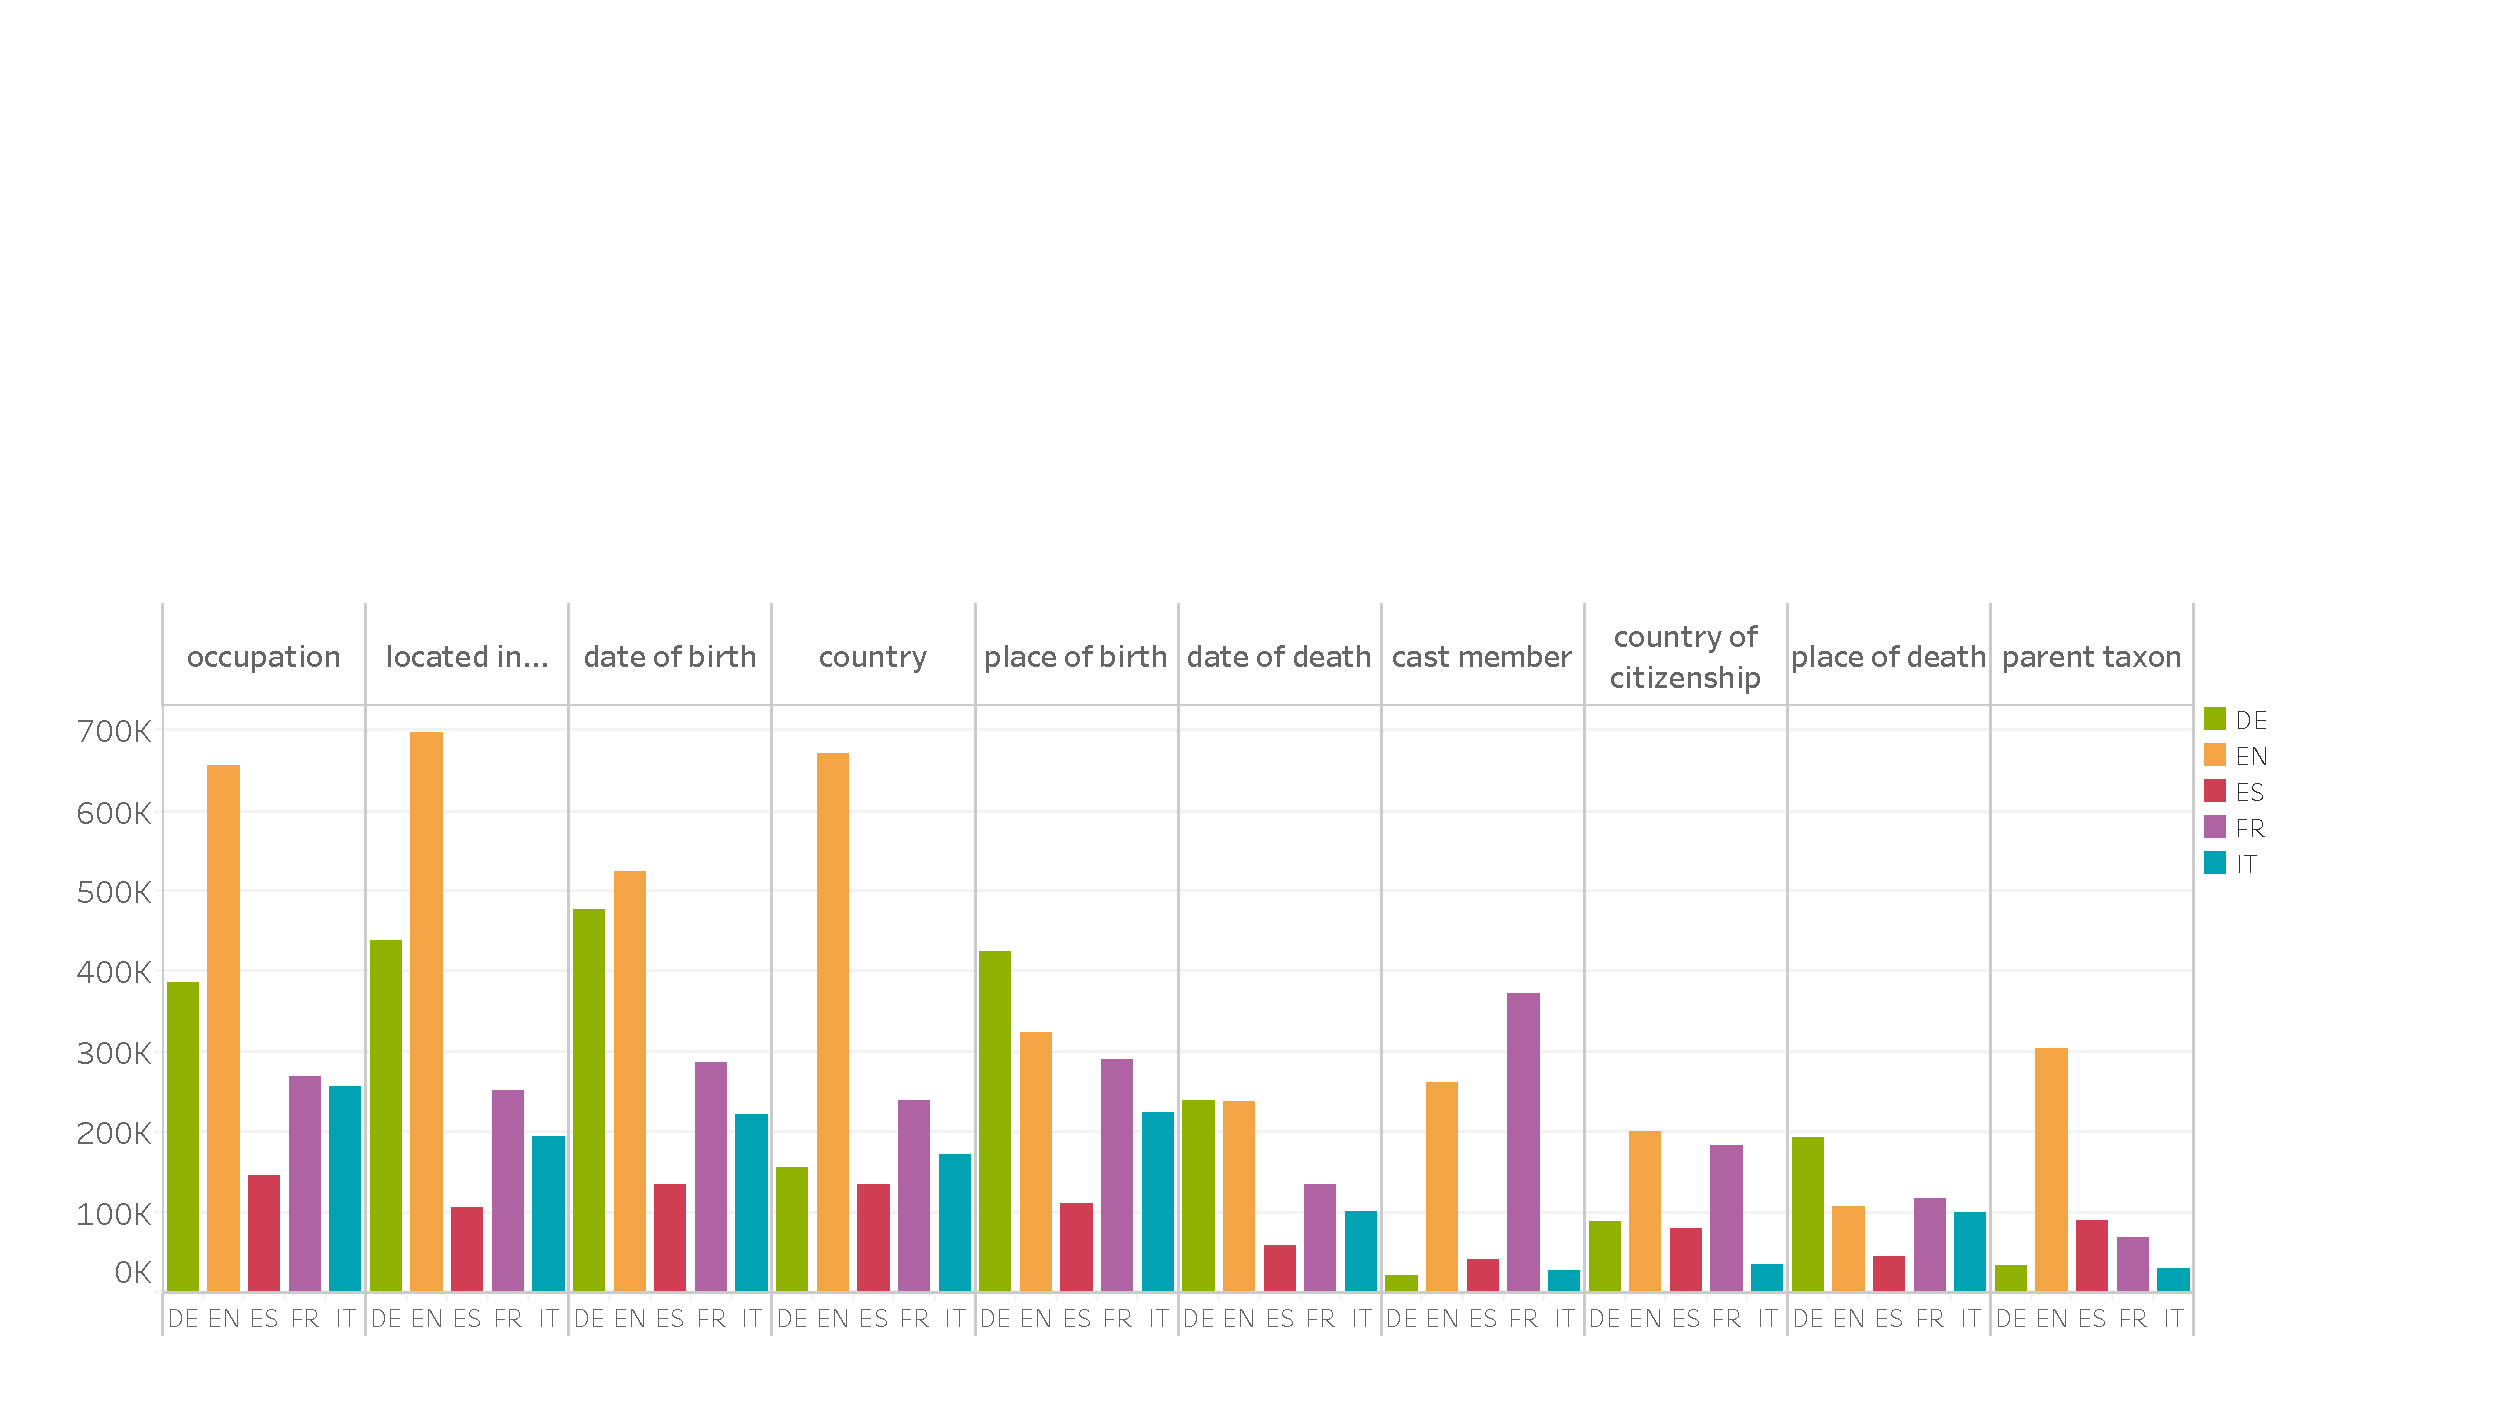
\includegraphics[width=\textwidth]{images/count_examples-property_per_language_wide.pdf}
\caption{The number of triples for the top 10 properties in each language.}
\label{fig:top_10}
\end{figure}
\chapter{Method}
\label{chpt:5}

\paragraph{}
In the 

\section{NAMANDA}
\section{Cross-Lingual Model Transfer}


\section{One Model, Multiple Languages}


\chapter{Experiments}
\paragraph{}
In this chapter we take an overview of the experiments that we used to evaluate our system. We analyze the results, and present some problems of our approach. Finally we compare our system with some state-of-the-art solutions.


\section{Dataset}
\chapter{Conclusions}
\label{chpt:7}
\paragraph{}
Given the widely lamented fact that KBs and resources are highly skewed towards English causing difficulties in the development of NLP system for low-resource languages, in this thesis we introduced a new large-scale multilingual dataset (\textbf{X-WikiRE}) for relation extraction. It is a reading comprehension-based relation extraction dataset for five languages: English, German, French, Spanish, and Italian. We hope that \textbf{X-WikiRE} will facilitate the research on multilingual methods for relation extraction. \textbf{X-WikiRE} is at least an order of magnitude larger than previous multilingual datasets. We used \textbf{X-WikiRE} to  experiment with various transfer learning setup using a state-of-the-art nil-aware machine reading comprehension model to perform zero-shot relation extraction. We evaluated the use of our resource using two different setups: transfer learning and joint learning. The experiments demonstrated that: \begin{enumerate}[a) , font=\bfseries, noitemsep]
    \item  multilingual training can be employed to exploit the fact that KBs are better populated in different areas for different languages, providing a strong cross-lingual supervision signal which leads to considerably better zero-shot relation extraction;
    \item models can be transferred cross-lingually with a minimal amount of target language data for fine-tuning;
    \item better modelling of nil-awareness in reading comprehension models leads to improvements on the task.
\end{enumerate}

Our work is a step towards making KBs equally well-resourced across languages. Future work may include the use of better multilingual embeddings with higher coverage, as we saw affects the performances in the zero-shot scenario drastically. Moreover, it will be interesting to expand the dataset to more languages, in particular to true low-resourced ones. 


% Our dataset covers more languages (five) and is at least an order of magnitude larger than existing multilingual RE datasets, e.g., TAC 2016 \citep{ellis2015overview}, which covers three languages and consists of $\approx$ 90k examples. We also a) perform cross-lingual RE showing that models pretrained on one language can be effectively transferred to others with minimal in-language finetuning; b) leverage multilingual representations to train a model capable of simultaneously performing (zero-shot) RE in all five languages, rivaling or outperforming its monolingually trained counterparts in many cases while requiring far fewer parameters per language; c) obtain considerable improvements by employing a more carefully designed nil-aware machine comprehension model. 

\bibliography{references}

 

\end{document}